\documentclass[10pt,a4paper,twocolumn]{article}

%====================================================
% PACKAGES
%====================================================
\usepackage[a4paper, top=2cm, bottom=2cm, left=1.5cm, right=1.5cm,
            columnsep=0.6cm]{geometry}
\usepackage{times}
\usepackage{microtype}
\usepackage{graphicx}
\usepackage{float}
\usepackage{booktabs}
\usepackage{array}
\usepackage{longtable}
\usepackage{caption}
\usepackage{subcaption}
\usepackage{amsmath}
\usepackage{amssymb}
\usepackage{setspace}
\usepackage{hyperref}
\usepackage{xcolor}
\usepackage{fancyhdr}
\usepackage{titlesec}
\usepackage{abstract}
\usepackage{enumitem}
\usepackage{parskip}

%====================================================
% TYPOGRAPHY AND SPACING
%====================================================
\setlength{\parskip}{1pt}
\setlength{\parindent}{1em}
\captionsetup{font=small, labelfont=bf, skip=4pt}
\setlength{\textfloatsep}{6pt}
\setlength{\floatsep}{4pt}
\setlength{\intextsep}{4pt}

% Section heading styles — compact, professional
\titleformat{\section}
  {\normalfont\normalsize\bfseries\scshape}
  {\Roman{section}.}{0.5em}{}
\titlespacing{\section}{0pt}{6pt}{2pt}

\titleformat{\subsection}
  {\normalfont\normalsize\itshape}
  {\Alph{subsection}.}{0.4em}{}
\titlespacing{\subsection}{0pt}{4pt}{1pt}

% Abstract formatting
\renewcommand{\abstractnamefont}{\normalfont\bfseries\scshape\normalsize}
\setlength{\absleftindent}{0pt}
\setlength{\absrightindent}{0pt}
\setlength{\abstitleskip}{-\parskip}
\abslabeldelim{\textbf{---}}

%====================================================
% HEADER / FOOTER
%====================================================
\pagestyle{fancy}
\fancyhf{}
\fancyhead[L]{\small\textit{Global Financial Market Analysis: 2000--2026}}
\fancyhead[R]{\small\textit{Sagnik Kundu}}
\fancyfoot[C]{\small\thepage}
\renewcommand{\headrulewidth}{0.4pt}

%====================================================
% HYPERREF
%====================================================
\hypersetup{
  colorlinks=true,
  linkcolor=black,
  citecolor=black,
  urlcolor=blue
}

%====================================================
% DOCUMENT
%====================================================
\begin{document}

%====================================================
% TITLE BLOCK
%====================================================
\twocolumn[{
\begin{center}
  {\Large\bfseries Global Financial Market Analysis: 2000--May 2026}\\[0.6em]
  {\normalsize\textit{A Comprehensive Exploratory Study of Multi-Asset Historical Market Data}}\\[1em]
  {\normalsize\textbf{Sagnik Kundu}}\\[0.2em]
  {\small June 2026}
\end{center}

\vspace{0.6em}
\hrule
\vspace{0.4em}

\begin{abstract}
\noindent
This paper presents a comprehensive exploratory data analysis (EDA) of a global financial
market dataset comprising 187,611 observations spanning from January 2000 to May 2026,
covering four major asset classes: stock indices, commodities, currencies, and cryptocurrencies.
The study investigates market composition, long-term price trajectories, inter-variable
correlations, and the influence of major macroeconomic events including the Dot-Com Crash
(2000--2002), the Global Financial Crisis (2007--2009), and the COVID-19 pandemic (2020).
A structured analytical workflow encompassing data preprocessing, temporal analysis, moving
average modeling, and correlation heatmap construction was employed using Python-based tools
(Pandas, NumPy, Matplotlib, Seaborn). Results indicate that while stock indices dominate
the dataset by record count, cryptocurrencies exhibit disproportionately high trading volumes
and have emerged as a dominant force in post-2017 market dynamics. Long-term trend analysis
confirms sustained market growth punctuated by event-driven disruptions, with the post-2020
period recording the most pronounced growth phase. Strong positive correlations among OHLC
(Open, High, Low, Close) variables and a structurally distinct behavior of trading volume
are also documented.

\smallskip\noindent\textbf{Keywords:} Financial Markets, Exploratory Data Analysis, Time-Series Analysis,
Cryptocurrency, Moving Averages, Market Events, OHLC Data.
\end{abstract}

\vspace{0.4em}
\hrule
\vspace{1em}
}]

%====================================================
% SECTION I: INTRODUCTION
%====================================================
\section{Introduction}

Financial markets are central to the functioning of the global economy, enabling capital allocation, price discovery, and risk distribution across asset classes and geographies. The period from 2000 to 2026 represents one of the most turbulent and transformative eras in modern financial history, encompassing the collapse of the technology bubble, a global credit crisis, a pandemic-induced market shock, and the rapid ascent of cryptocurrency as a legitimate asset class.

Exploratory analysis of long-horizon market data allows researchers and practitioners to identify structural patterns, quantify volatility regimes, and understand how different asset categories respond to macroeconomic shocks. Unlike predictive modeling, EDA aims to surface latent structure within the data—revealing distributional characteristics, temporal trends, and cross-variable relationships that inform subsequent modeling or policy analysis.

\subsection{Motivation}

Existing literature on financial market analysis often focuses on single asset classes or short time windows. Multi-asset, multi-decade analyses are comparatively rare, despite being highly informative for portfolio construction, systemic risk assessment, and understanding secular trends in global capital markets.

\subsection{Objectives}

The primary objectives of this study are:
\begin{itemize}[leftmargin=1.2em, itemsep=1pt, topsep=2pt]
  \item To characterize the composition and structure of a multi-asset financial dataset.
  \item To perform rigorous data quality assessment and cleaning prior to analysis.
  \item To investigate trading volume dynamics across asset classes.
  \item To evaluate long-term price trends using multiple temporal aggregations and moving averages.
  \item To assess the temporal impact of major macroeconomic events on market prices.
  \item To quantify relationships among OHLC price variables and trading volume.
\end{itemize}

\subsection{Scope and Limitations}

This study is restricted to exploratory and descriptive analysis. Predictive modeling, volatility forecasting, and causal inference are considered future work. The dataset is treated as a representative sample; survivorship bias and selection effects inherent to the data source are acknowledged but not corrected. The seven consistency anomalies identified during data cleaning (Section~IV-B) were retained with documentation rather than removed or imputed, preserving the integrity of extreme-market-event records.

%====================================================
% SECTION II: DATASET DESCRIPTION
%====================================================
\section{Dataset Description}

\subsection{Overview}

The dataset is sourced from Kaggle and contains historical daily market records across multiple asset classes and geographic regions. Key attributes of the dataset are summarized in Table~\ref{tab:dataset_summary}.

\begin{table}[H]
\centering
\caption{Dataset Summary Statistics}
\label{tab:dataset_summary}
\small
\begin{tabular}{@{}ll@{}}
\toprule
\textbf{Attribute} & \textbf{Value} \\
\midrule
Total Records       & 187,611 \\
Total Features      & 10 \\
Unique Assets       & 34 \\
Time Period         & Jan 2000 -- May 2026 \\
Total Years         & $\approx$ 26.4 \\
Asset Classes       & 4 \\
Numerical Features  & Open, High, Low, Close, Volume \\
Missing Values      & None detected \\
Duplicate Records   & None detected \\
Memory Usage        & 14.3 MB \\
\bottomrule
\end{tabular}
\end{table}

\subsection{Feature Description}

Each record represents a single trading day for a given financial instrument and includes the following fields: \textit{Open} (opening price), \textit{High} (intraday high), \textit{Low} (intraday low), \textit{Close} (closing price), and \textit{Volume} (total units traded). The \textit{Date} column was stored as a \texttt{string} in the raw file and was coerced to \texttt{datetime64[us]} during preprocessing. Categorical identifiers include \textit{symbol} (ticker), \textit{asset\_name}, \textit{asset\_type}, and \textit{region}.

\subsection{Asset Classes}

The dataset covers four asset categories:
\begin{itemize}[leftmargin=1.2em, itemsep=1pt, topsep=2pt]
  \item \textbf{Stock Indices:} Broad market benchmarks (e.g., S\&P 500, NASDAQ, FTSE 100, Nikkei 225, SENSEX, HSI) —- 63,610 records.
  \item \textbf{Commodities:} Physical goods including Gold, Brent Crude, and WTI Crude Oil —- 49,965 records.
  \item \textbf{Currencies:} Major and minor forex pairs (EUR/USD, JPY/USD, etc.) —- 47,629 records.
  \item \textbf{Cryptocurrencies:} Digital assets including Bitcoin, Ethereum, Ripple, Solana, Litecoin, and Dogecoin —- 26,407 records.
\end{itemize}

The record distribution reflects the differential availability of historical data: traditional asset classes have uninterrupted coverage from January 2000, while most cryptocurrency records begin after 2013 (Bitcoin) or after 2017 for other cryptocurrencies.

%====================================================
% SECTION III: DATA CLEANING AND PREPROCESSING
%====================================================
\section{Data Cleaning \& Preprocessing}

\subsection{Missing Value Analysis}

A complete column-wise null audit was conducted using \texttt{DataFrame.isnull().sum()}. The result confirmed that \textbf{zero missing values} exist across all 10 features and all 187,611 records. No imputation or row-dropping was required. This represents a high baseline data quality, uncommon in real-world financial datasets of comparable size and multi-source composition.

\subsection{Duplicate Record Detection}

A full-row duplicate check via \texttt{DataFrame.duplicated().sum()} returned zero duplicates, indicating that each observation is a distinct (date, asset) pairing. No de-duplication step was necessary prior to analysis.

\subsection{Date Type Coercion}

The \textit{date} column was originally stored as a Python \texttt{str} object. It was converted to \texttt{datetime64[us]} using \texttt{pd.to\_datetime()}, enabling downstream operations including temporal resampling, rolling window computations, and chronological sorting. Table~\ref{tab:dtype_change} summarizes the type change.

\begin{table}[H]
\centering
\caption{Date Column Type Conversion}
\label{tab:dtype_change}
\small
\begin{tabular}{@{}lll@{}}
\toprule
\textbf{Column} & \textbf{Before} & \textbf{After} \\
\midrule
date & \texttt{str} & \texttt{datetime64[us]} \\
\bottomrule
\end{tabular}
\end{table}

\subsection{Data Consistency Checks}

Two logical constraints were validated:

\textbf{High $\geq$ Low Invariant.} The condition \texttt{df["high"] < df["low"]} identified \textbf{7 violated records}. These were predominantly commodity observations (Gold and Brent Crude, 2009--2010), accounting for less than 0.004\% of the dataset. As summarized in Table~\ref{tab:anomalies}, they were retained and flagged rather than removed, since the anomalies likely reflect data entry artefacts in thinly traded sessions rather than systematic error.

\begin{table}[H]
\centering
\caption{High/Low Inconsistency Records}
\label{tab:anomalies}
\small
\begin{tabular}{@{}llll@{}}
\toprule
\textbf{Date} & \textbf{Symbol} & \textbf{Asset} & \textbf{High} \\
\midrule
2009-11-23 & GC=F & Gold        & 1163.00 \\
2009-12-23 & BZ=F & Brent Crude & 75.13 \\
2009-12-24 & BZ=F & Brent Crude & 75.93 \\
2010-01-04 & BZ=F & Brent Crude & 79.82 \\
2010-01-05 & BZ=F & Brent Crude & 80.26 \\
2010-01-07 & BZ=F & Brent Crude & 81.51 \\
2010-04-15 & BZ=F & Brent Crude & 87.13 \\
\bottomrule
\end{tabular}
\end{table}

\textbf{Negative Price Records.} The \textit{open} column contains exactly one negative value (\texttt{-14.00}) and the \textit{close} column one negative value (\texttt{-37.63}), both corresponding to WTI Crude Oil (\texttt{CL=F}) on \textbf{21 April 2020}. This date coincides with the historically unprecedented event in which front-month WTI futures settled at negative prices owing to storage capacity constraints during the COVID-19 demand collapse. These records are valid representations of realized market conditions and were retained without modification.

\subsection{Cleaning Summary}

Table~\ref{tab:cleaning_summary} provides a consolidated record of all cleaning actions taken.

\begin{table}[H]
\centering
\caption{Data Cleaning Action Log}
\label{tab:cleaning_summary}
\small
\begin{tabular}{@{}p{3cm}p{4cm}@{}}
\toprule
\textbf{Check} & \textbf{Outcome} \\
\midrule
Missing values      & None; no action required \\
Duplicate records   & None; no action required \\
Date type coercion  & \texttt{str} $\rightarrow$ \texttt{datetime64[us]} \\
High/Low anomalies  & 7 records flagged; retained \\
Negative prices     & 1 WTI record; valid, retained \\
Negative volume     & None detected \\
\bottomrule
\end{tabular}
\end{table}

The cleaned dataset was exported to \texttt{processed/cleaned\_market\_data.csv} for use in all downstream analysis notebooks.

%====================================================
% SECTION IV: METHODOLOGY
%====================================================
\section{Methodology}

\subsection{Analytical Workflow}

The analysis followed a structured eight-stage pipeline designed to move progressively from raw data ingestion to insight generation:

\begin{enumerate}[leftmargin=1.4em, itemsep=1pt, topsep=2pt]
  \item \textbf{Data Understanding:} Schema inspection, data type assessment, and feature profiling.
  \item \textbf{Data Cleaning:} Duplicate removal, null imputation assessment, and type coercion.
  \item \textbf{Date Parsing:} Conversion of string dates to \texttt{datetime} objects; extraction of year, month, and quarter features.
  \item \textbf{Exploratory Data Analysis:} Distribution analysis, volume profiling, and asset-class characterization.
  \item \textbf{Time-Series Analysis:} Daily, monthly, quarterly, and yearly aggregation of closing prices.
  \item \textbf{Moving Average Analysis:} Computation of 12-month and 24-month rolling averages on the monthly close series.
  \item \textbf{Correlation Analysis:} Pearson correlation matrix for all numerical variables.
  \item \textbf{Market Event Analysis:} Segmentation of the time series at key macroeconomic event boundaries.
\end{enumerate}

\subsection{Tools and Libraries}

All analyses were conducted in Python 3.11 within a Jupyter Notebook environment. Core libraries used include:
\begin{itemize}[leftmargin=1.2em, itemsep=1pt, topsep=2pt]
  \item \textbf{Pandas} -- Data wrangling, time-series resampling, and GroupBy operations.
  \item \textbf{NumPy} -- Numerical computation and array manipulation.
  \item \textbf{Matplotlib / Seaborn} -- Visualization (line plots, bar charts, heatmaps).
\end{itemize}

\subsection{Temporal Aggregation Scheme}

Four aggregation frequencies were applied to the closing price series to examine trends at different granularities:

\begin{equation}
  \bar{P}_{\Delta}(t) = \frac{1}{|\mathcal{T}_{\Delta}(t)|} \sum_{d \in \mathcal{T}_{\Delta}(t)} P_d
\end{equation}

where $P_d$ is the daily close price, $\Delta \in \{\text{daily, monthly, quarterly, yearly}\}$, and $\mathcal{T}_{\Delta}(t)$ is the set of trading days within the aggregation window $t$.

\subsection{Moving Average Specification}

Two rolling averages were computed on the monthly mean close price series:
\begin{equation}
  \text{MA}_k(t) = \frac{1}{k} \sum_{i=0}^{k-1} \bar{P}_{t-i}
\end{equation}
where $\bar{P}_t$ denotes the monthly mean closing price at month $t$, and $k \in \{12, 24\}$ represents the window length in months. The 12-month MA captures medium-term momentum; the 24-month MA suppresses cyclical fluctuations to isolate the secular trend.

%====================================================
% SECTION V: RESULTS AND DISCUSSION
%====================================================
\section{Results and Discussion}

\subsection{Asset Class Composition}

The dataset encompasses 34 unique financial instruments across four asset classes. Figure~\ref{fig:asset_dist} illustrates the distribution of records by asset type.

\begin{figure}[H]
  \centering
  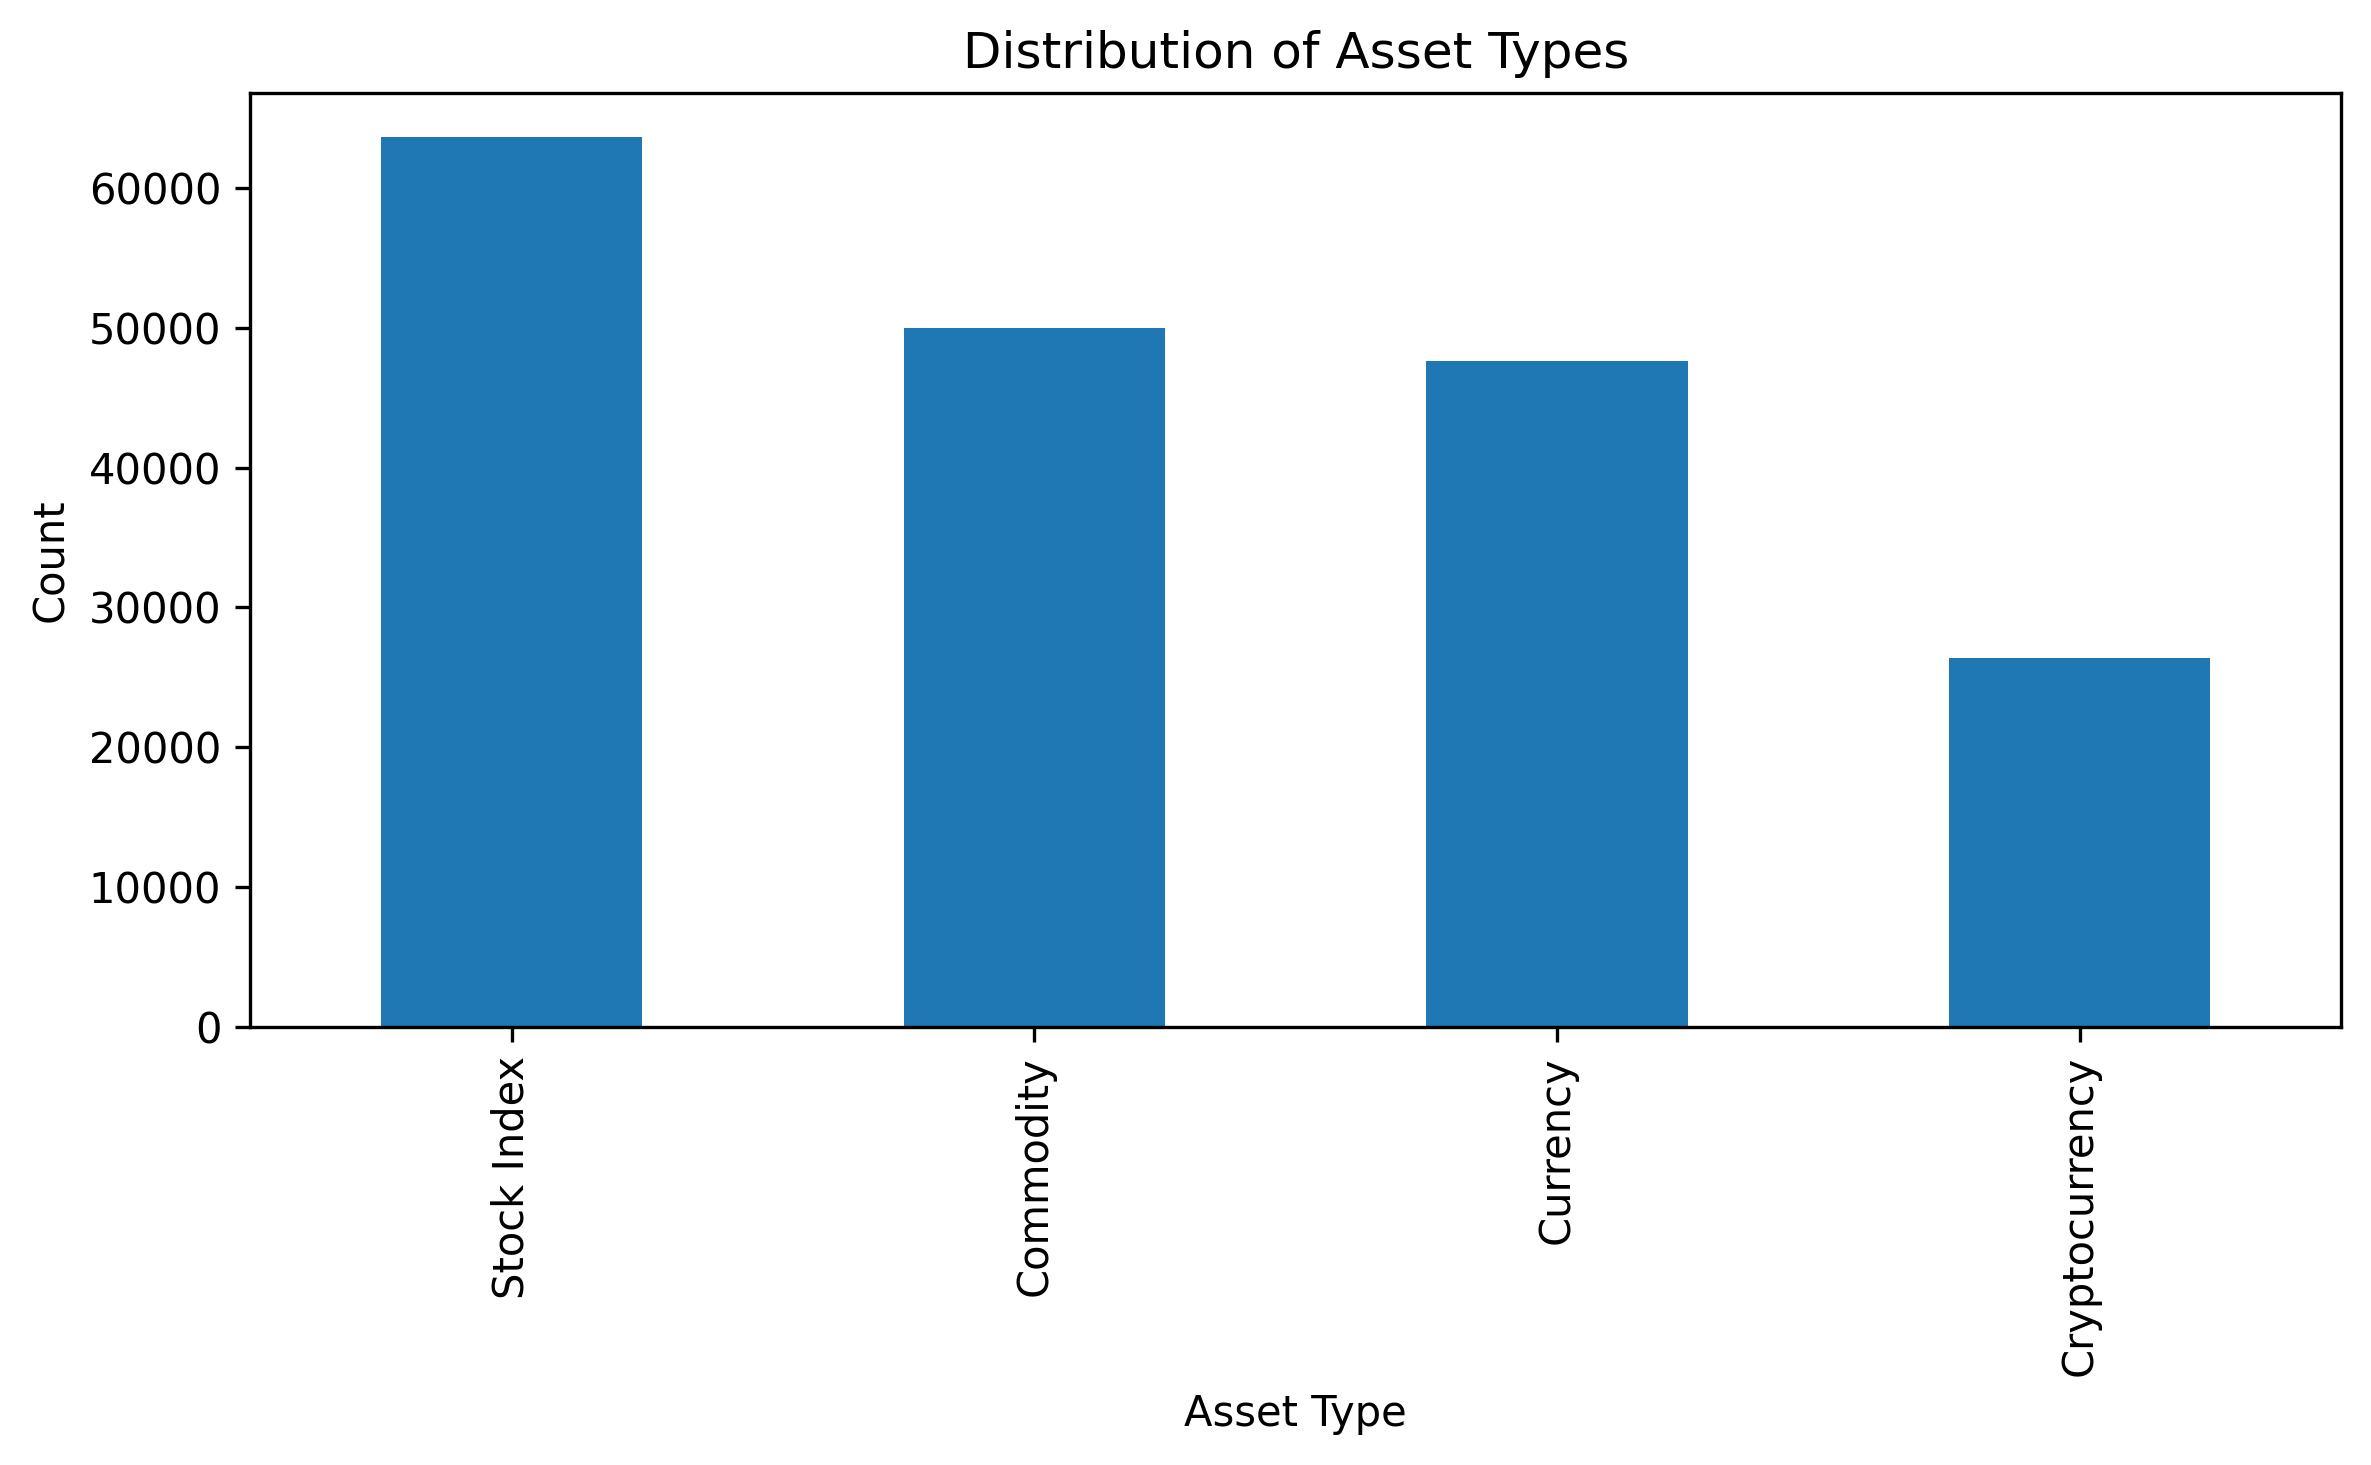
\includegraphics[width=\linewidth]{asset_distribution.png}
  \caption{Distribution of records by asset type. Stock indices account for the largest share (63,610 records), followed by commodities (49,965), currencies (47,629), and cryptocurrencies (26,407).}
  \label{fig:asset_dist}
\end{figure}

Stock indices constitute the largest single category by record count, reflecting the breadth of global equity benchmarks tracked over the full 26-year period. Cryptocurrencies represent the smallest share of observations due to their shorter market history. Bitcoin first appears in the dataset around 2013, while most other cryptocurrencies such as Ethereum, Ripple, Cardano, BNB, Solana, and Dogecoin enter after 2017.

The relative proportions highlight a structural asymmetry in the dataset: traditional asset classes have more complete historical coverage, while cryptocurrency records are concentrated in the more recent sub-period. This asymmetry must be acknowledged when interpreting any cross-class aggregate statistics.

\subsection{Records per Year}

The annual record count grows steadily from 3,124 in 2000 to peak values in excess of 8,500 in the 2020--2025 sub-period, reflecting the progressive expansion of the asset universe tracked in the dataset. Figure~\ref{fig:records_year} illustrates this trajectory.

\begin{figure}[H]
  \centering
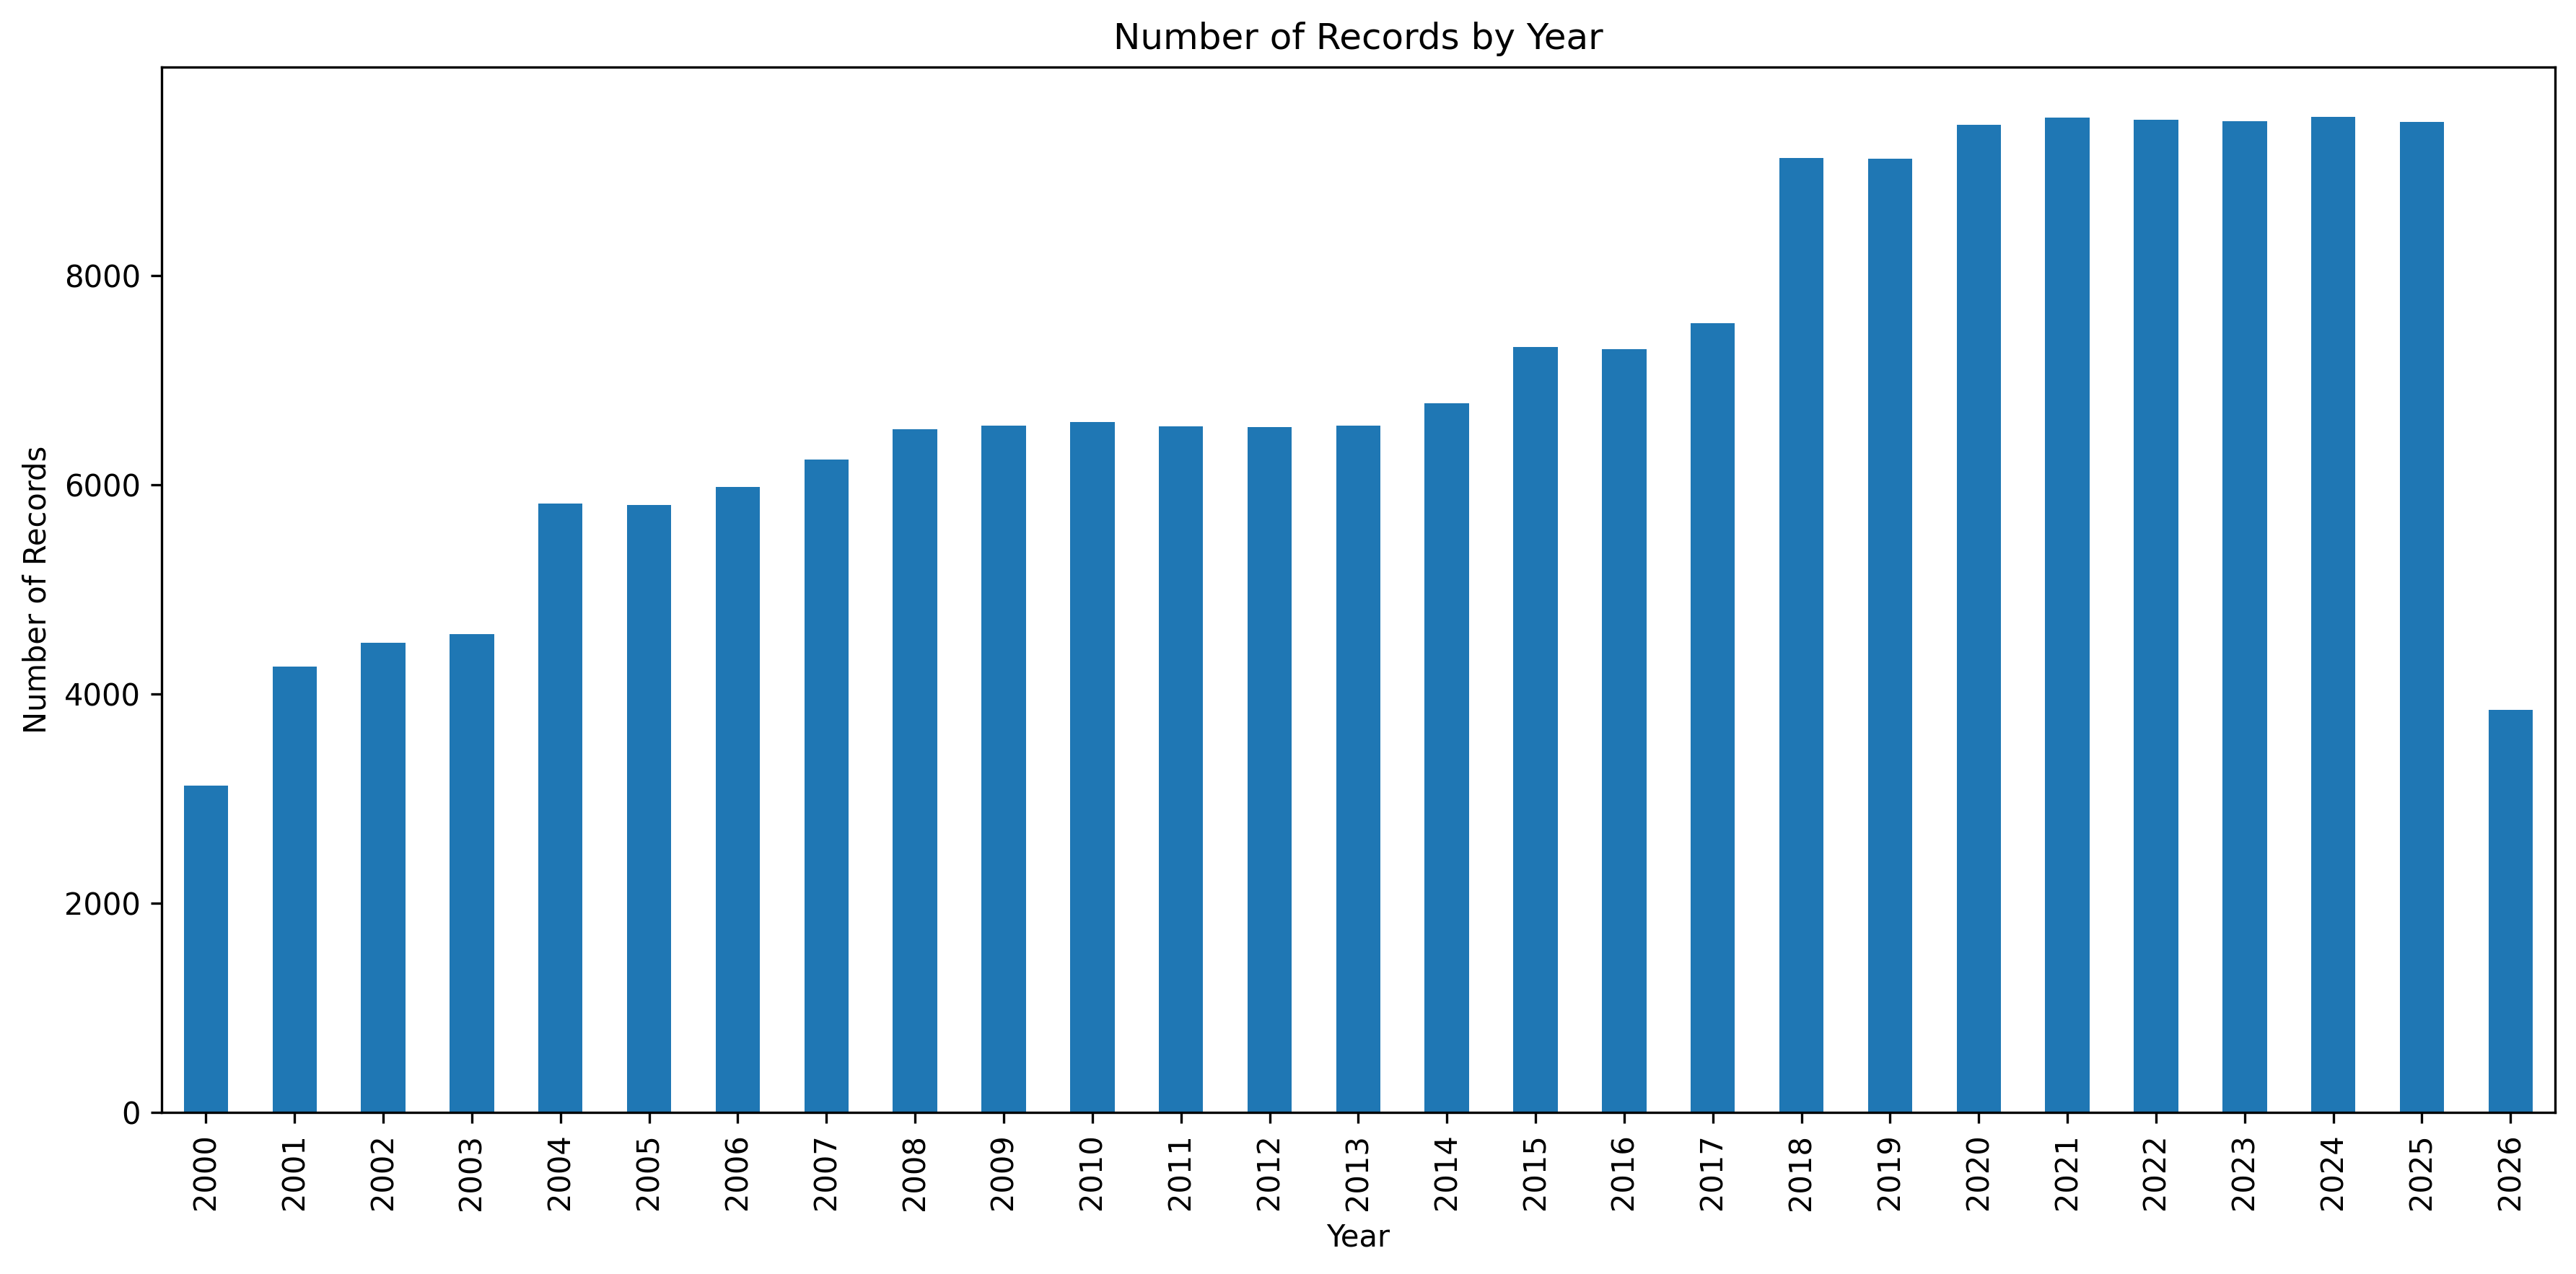
\includegraphics[width=\linewidth]{records_per_year.png}  
  \caption{Number of records per calendar year (2000--2026). The upward trend reflects the gradual addition of cryptocurrency instruments to the dataset from 2013 onward. The partial count for 2026 corresponds to data available through May only.}
  \label{fig:records_year}
\end{figure}

The partial count for 2026 (data available only through May) accounts for the apparent dip at the right-hand tail of the distribution.

\subsection{Trading Volume Analysis}

\textbf{Overall distribution.} The volume variable exhibits extreme right skew: the 25th percentile is zero, the median is approximately 71,800 units, and the maximum is $3.51 \times 10^{11}$. The interquartile range spans zero to $2.23 \times 10^8$, confirming that the majority of records correspond to low-volume instruments (currencies and smaller commodities) while a small number of cryptocurrency and equity-index records dominate total market activity. A log-transformed boxplot (Figure~\ref{fig:vol_box}) was used to visualise the full distribution without suppressing the lower-volume observations.

\begin{figure}[H]
  \centering
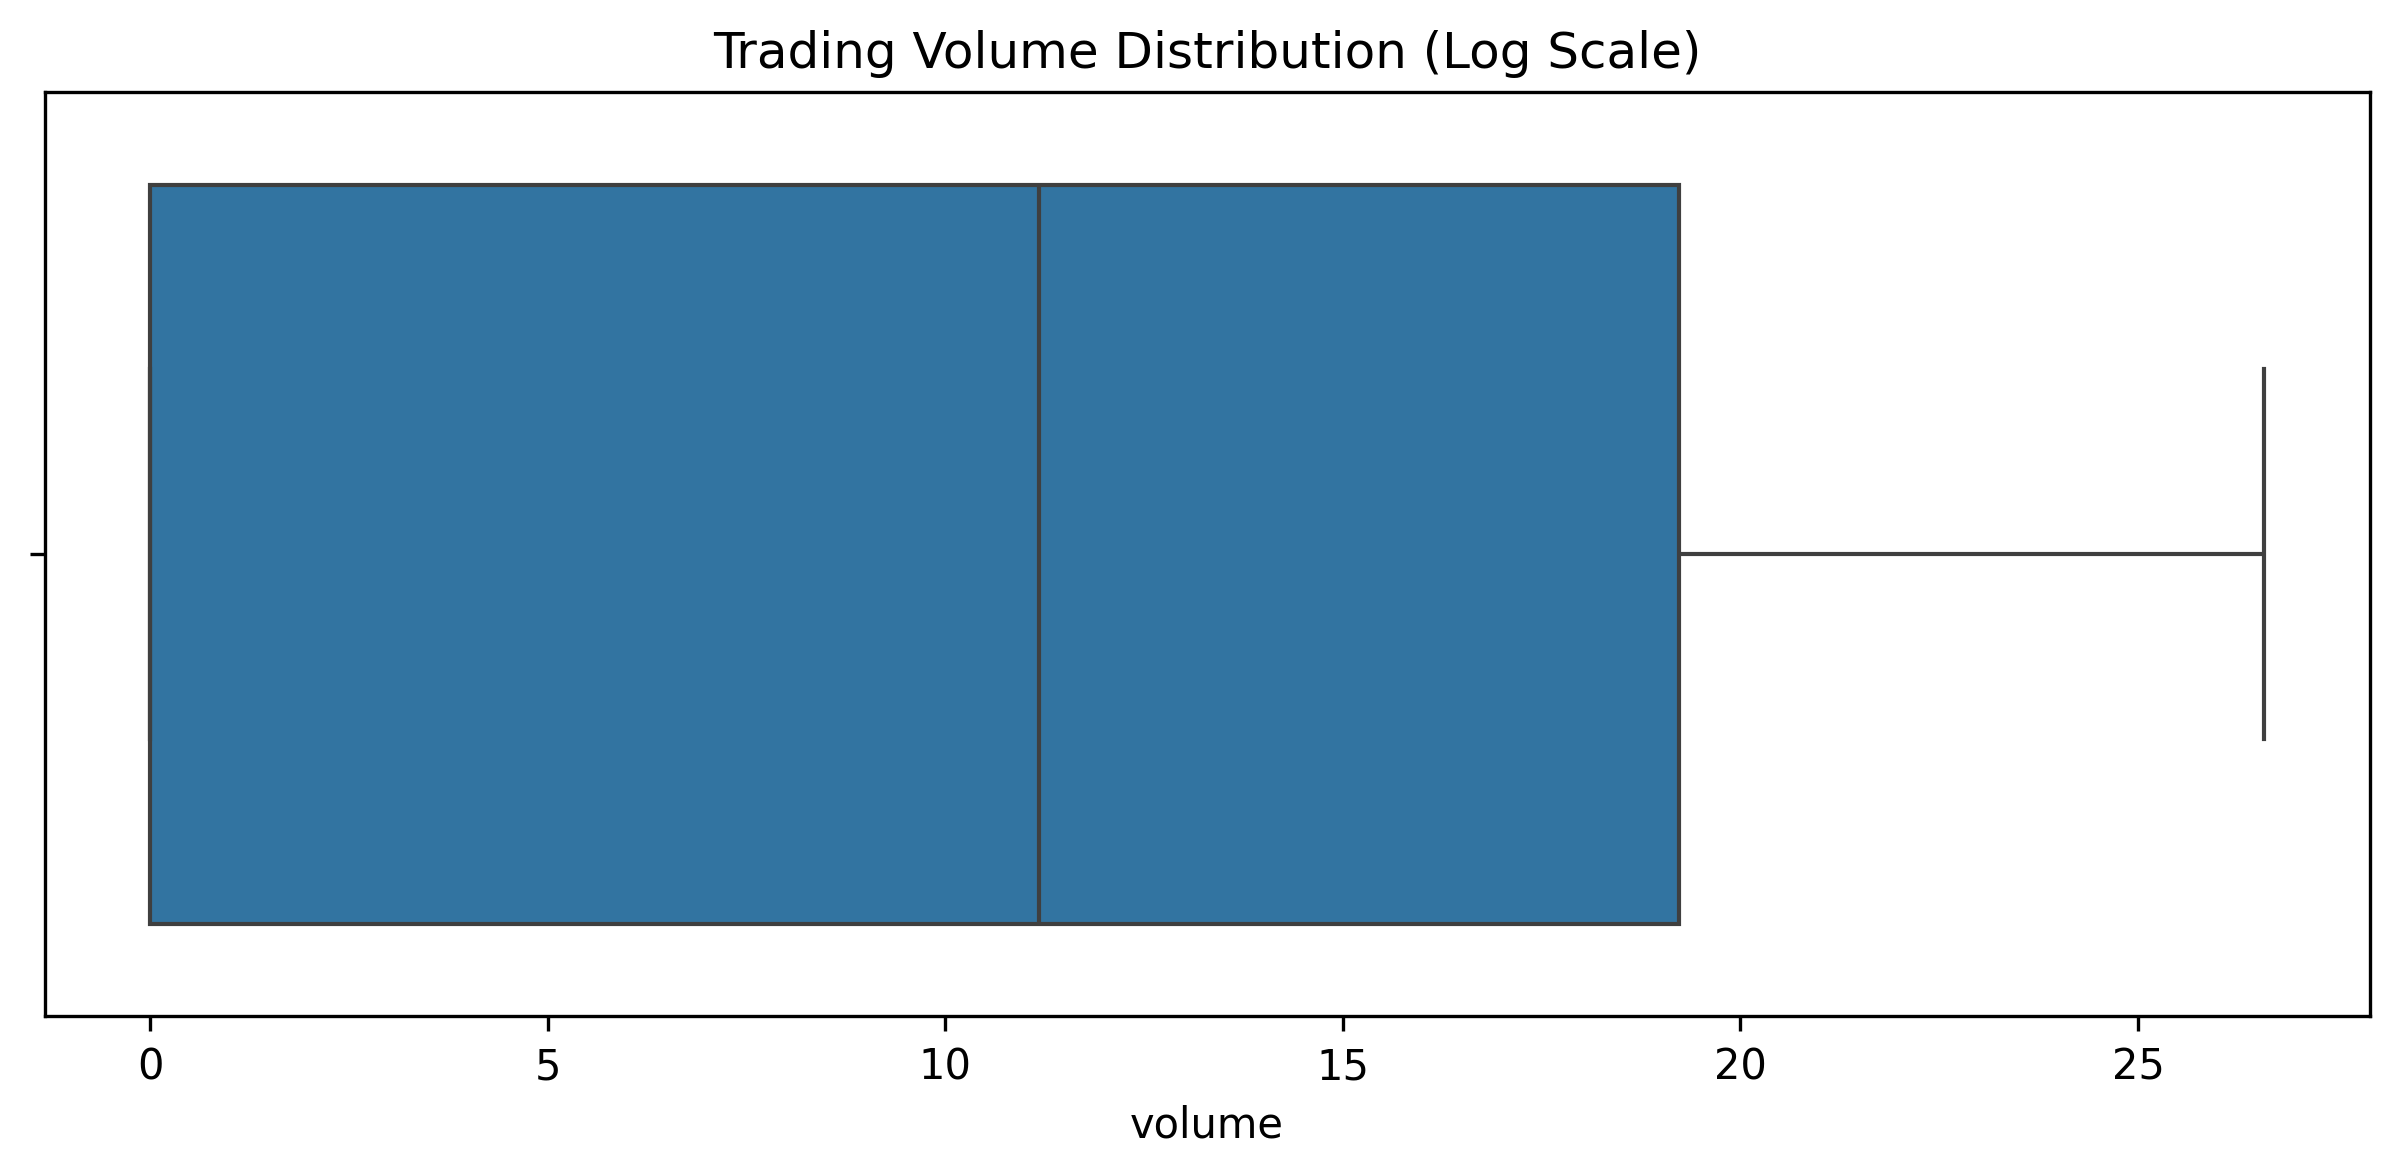
\includegraphics[width=\linewidth]{trading_volume.png}  \caption{Distribution of trading volume on a log-transformed scale ($\log_{e}(1 + \text{volume})$). The box reveals a wide interquartile range and numerous high-volume outliers corresponding to major cryptocurrency and equity-index sessions.}
  \label{fig:vol_box}
\end{figure}

\textbf{Top assets by total volume.} Table~\ref{tab:top_volume} and Figure~\ref{fig:top_vol_bar} present the ten highest-volume assets over the full study period.

\begin{table}[H]
\centering
\caption{Top 10 Assets by Total Cumulative Trading Volume}
\label{tab:top_volume}
\small
\begin{tabular}{@{}lll@{}}
\toprule
\textbf{Rank} & \textbf{Asset} & \textbf{Total Volume} \\
\midrule
1  & Bitcoin      & $9.51 \times 10^{13}$ \\
2  & Ethereum     & $4.75 \times 10^{13}$ \\
3  & S\&P 500     & $2.29 \times 10^{13}$ \\
4  & NASDAQ       & $1.91 \times 10^{13}$ \\
5  & HSI          & $1.05 \times 10^{13}$ \\
6  & Ripple       & $8.95 \times 10^{12}$ \\
7  & FTSE 100     & $7.06 \times 10^{12}$ \\
8  & Solana       & $5.40 \times 10^{12}$ \\
9  & Litecoin     & $5.19 \times 10^{12}$ \\
10 & Dogecoin     & $3.98 \times 10^{12}$ \\
\bottomrule
\end{tabular}
\end{table}

\begin{figure}[H]
  \centering
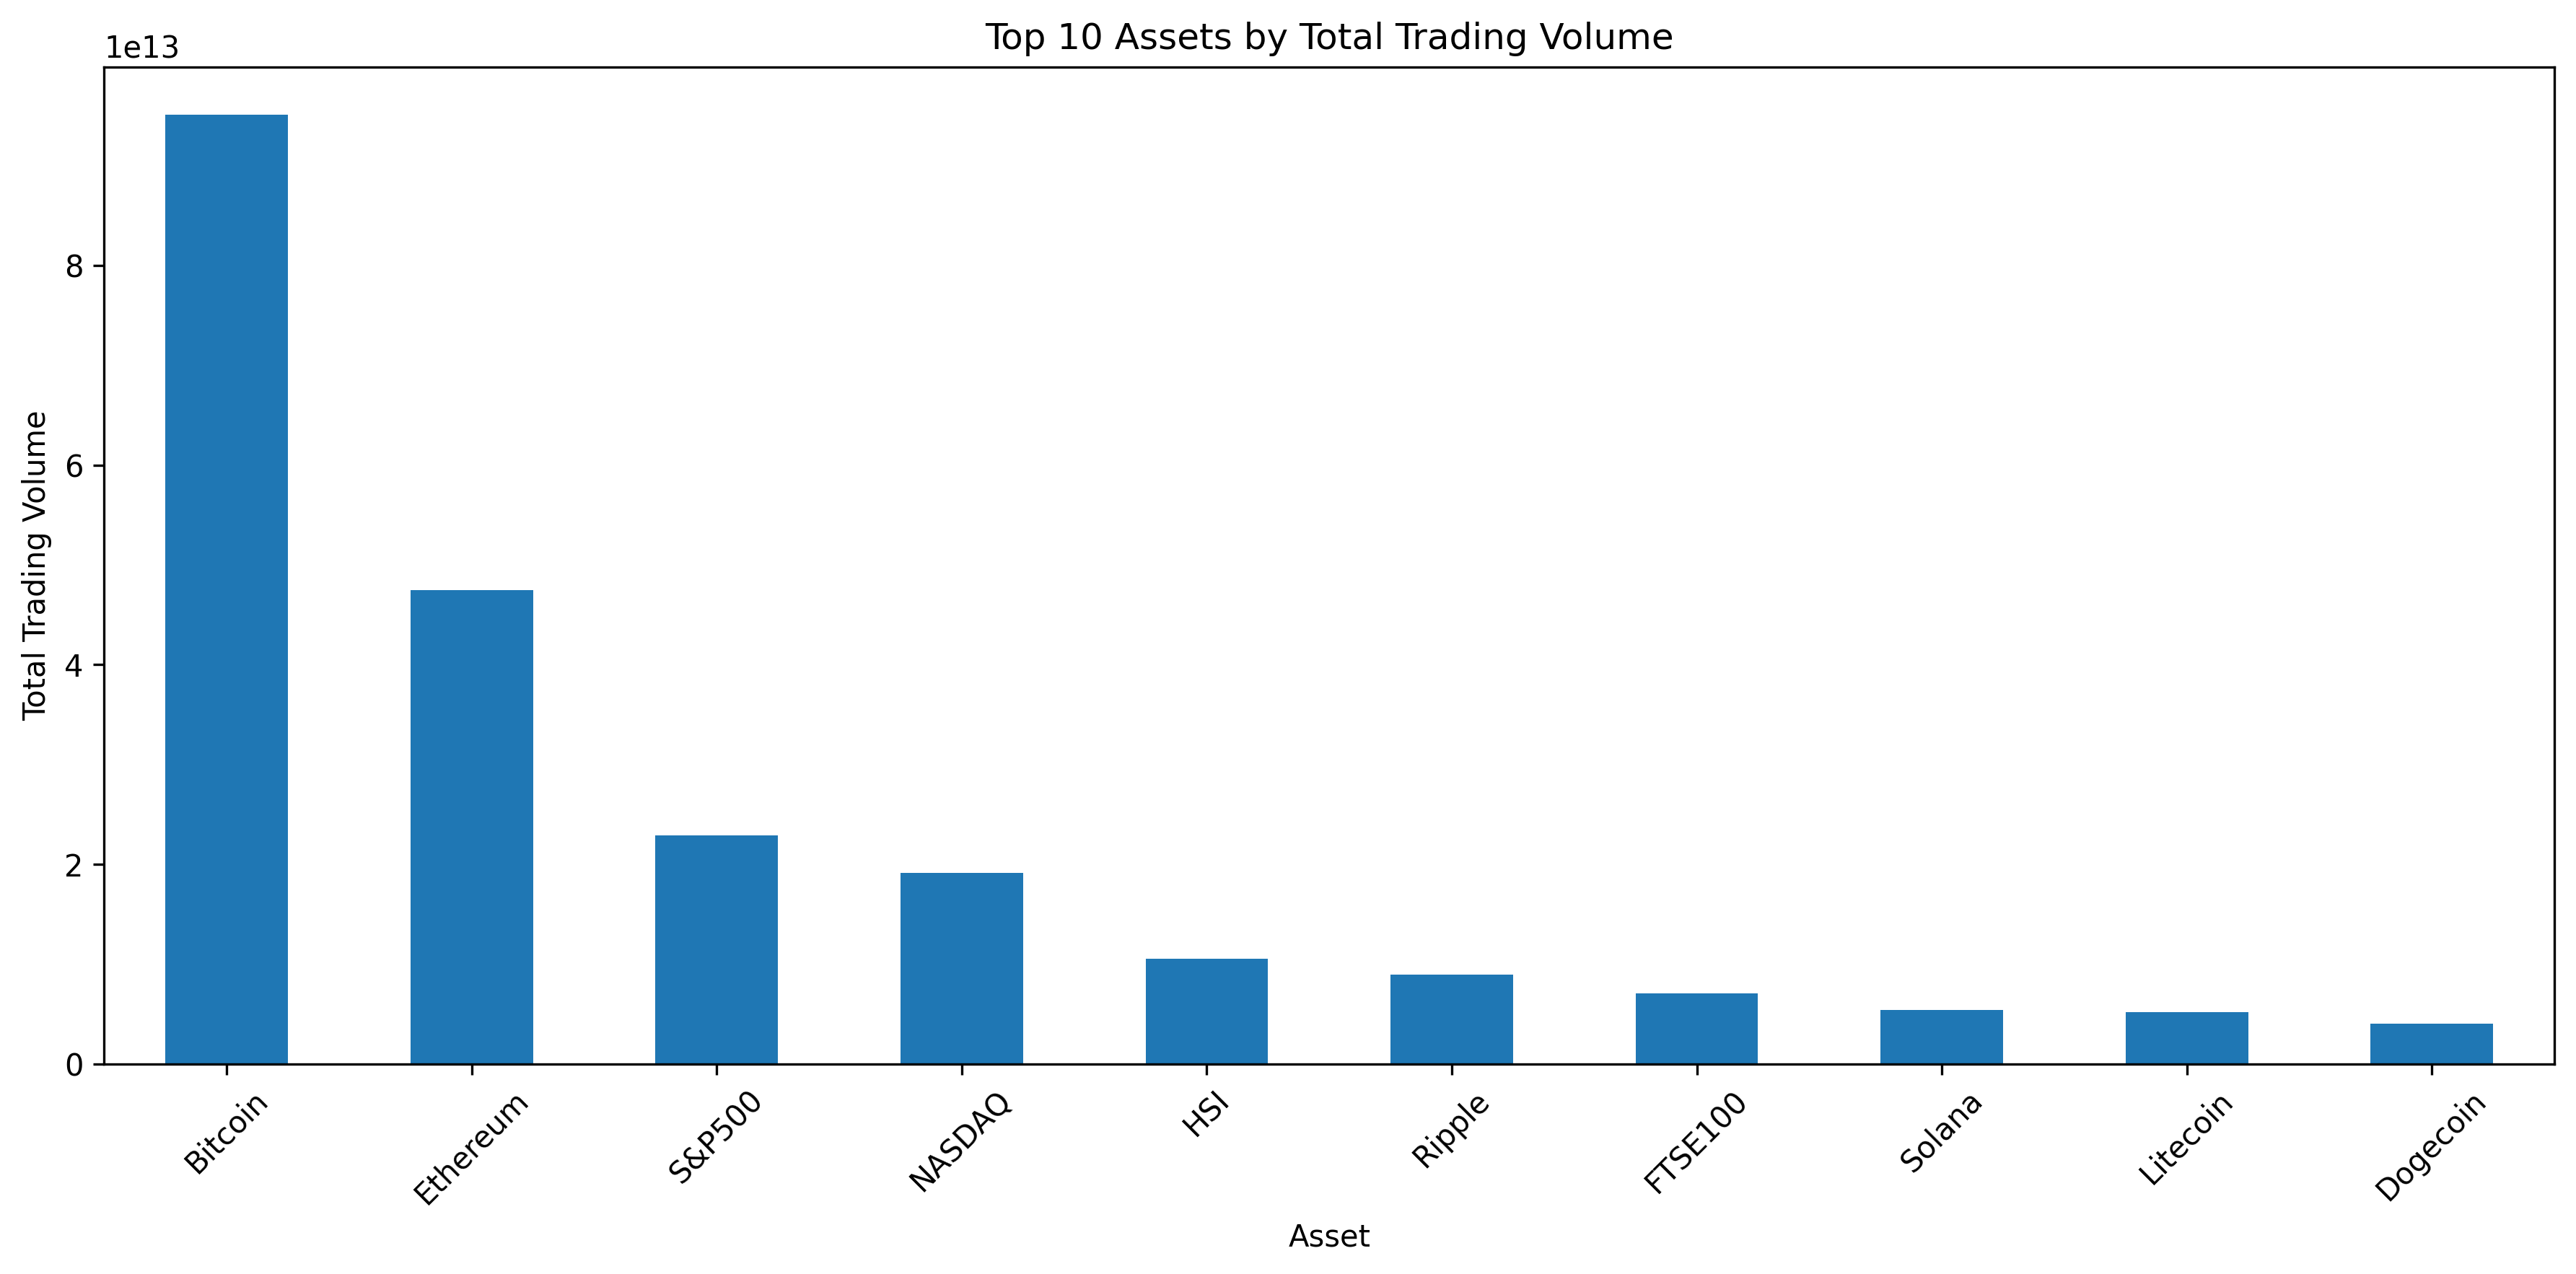
\includegraphics[width=\linewidth]{trading_volume_top10.png}  \caption{Total cumulative trading volume for the top 10 assets. Bitcoin's volume ($9.51 \times 10^{13}$) is approximately double that of Ethereum, which occupies second place. Six of the ten highest-volume assets are cryptocurrencies.}
  \label{fig:top_vol_bar}
\end{figure}

Bitcoin accounts for by far the largest cumulative volume in the dataset, approximately double that of Ethereum. The presence of Ripple, Solana, Litecoin, and Dogecoin among the top ten underscores the breadth of cryptocurrency market participation over the post-2017 sub-period.

\textbf{Average volume by asset class.} Figure~\ref{fig:avg_vol_type} and the values in Table~\ref{tab:avg_vol} reveal a pronounced volume hierarchy across asset classes.

\begin{table}[H]
\centering
\caption{Average Daily Trading Volume by Asset Class}
\label{tab:avg_vol}
\small
\begin{tabular}{@{}ll@{}}
\toprule
\textbf{Asset Type} & \textbf{Mean Daily Volume} \\
\midrule
Cryptocurrency & $6.55 \times 10^{9}$ \\
Stock Index    & $9.59 \times 10^{8}$ \\
Commodity      & $7.25 \times 10^{4}$ \\
Currency       & $0$ (reported) \\
\bottomrule
\end{tabular}
\end{table}

\begin{figure}[H]
  \centering
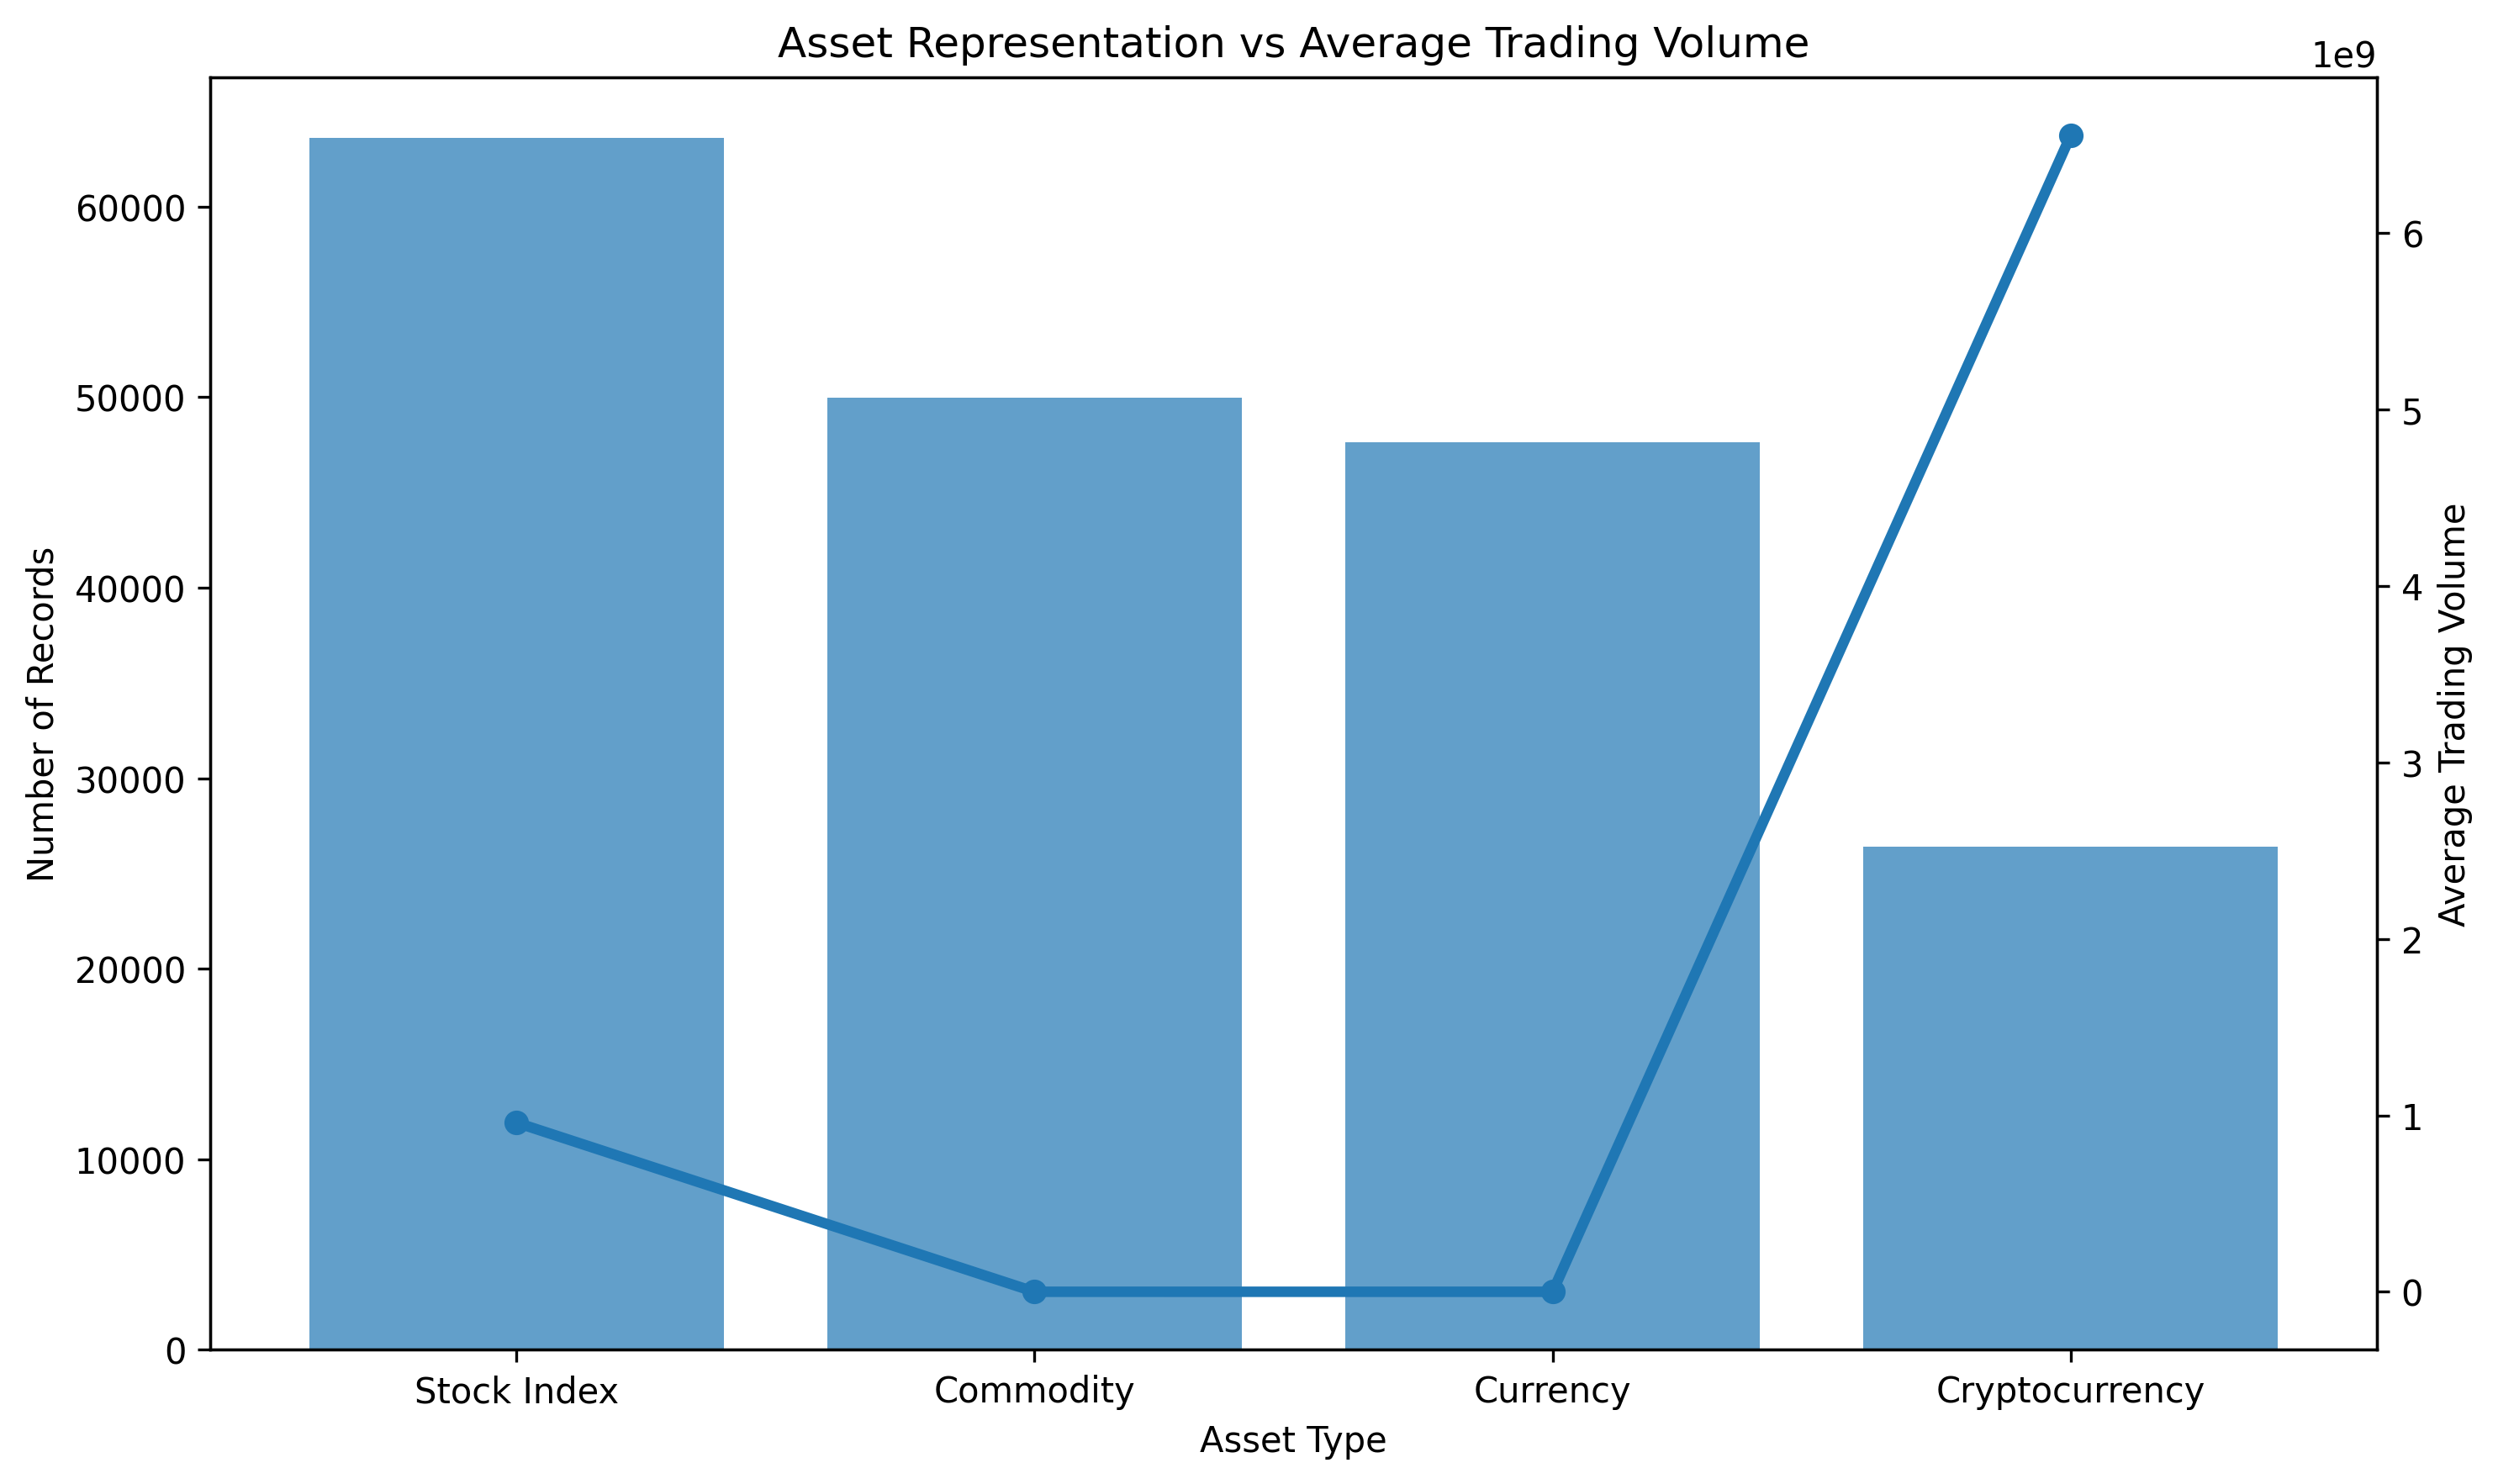
\includegraphics[width=\linewidth]{asset_vs_trading_volume.png}  \caption{Average daily trading volume by asset type (left axis, bars) overlaid with asset record count (right axis, line). Cryptocurrencies exhibit average volumes nearly seven times those of stock indices despite having the fewest records in the dataset.}
  \label{fig:avg_vol_type}
\end{figure}

Despite their lower representation, cryptocurrencies exhibit substantially higher average daily trading volumes compared to all other asset classes. This finding reflects the 24/7 market structure of cryptocurrency exchanges, the global retail participation base, and the speculative intensity that characterizes digital asset markets.

Traditional asset classes, particularly currencies and commodities, show comparatively moderate average volumes, while stock indices occupy an intermediate position. The concentration of trading activity within a small subset of high-volume assets (notably Bitcoin and Ethereum) further amplifies this disparity. This volume-representation divergence has important implications for any analysis that weights observations equally across asset classes.

\subsection{Multi-Horizon Time-Series Analysis}

Monthly aggregated closing prices reveal a strong secular upward trend spanning the full 2000--2026 window. Figure~\ref{fig:ts_4panel} presents the closing price series across four temporal resolutions.

\begin{figure}[H]
  \centering
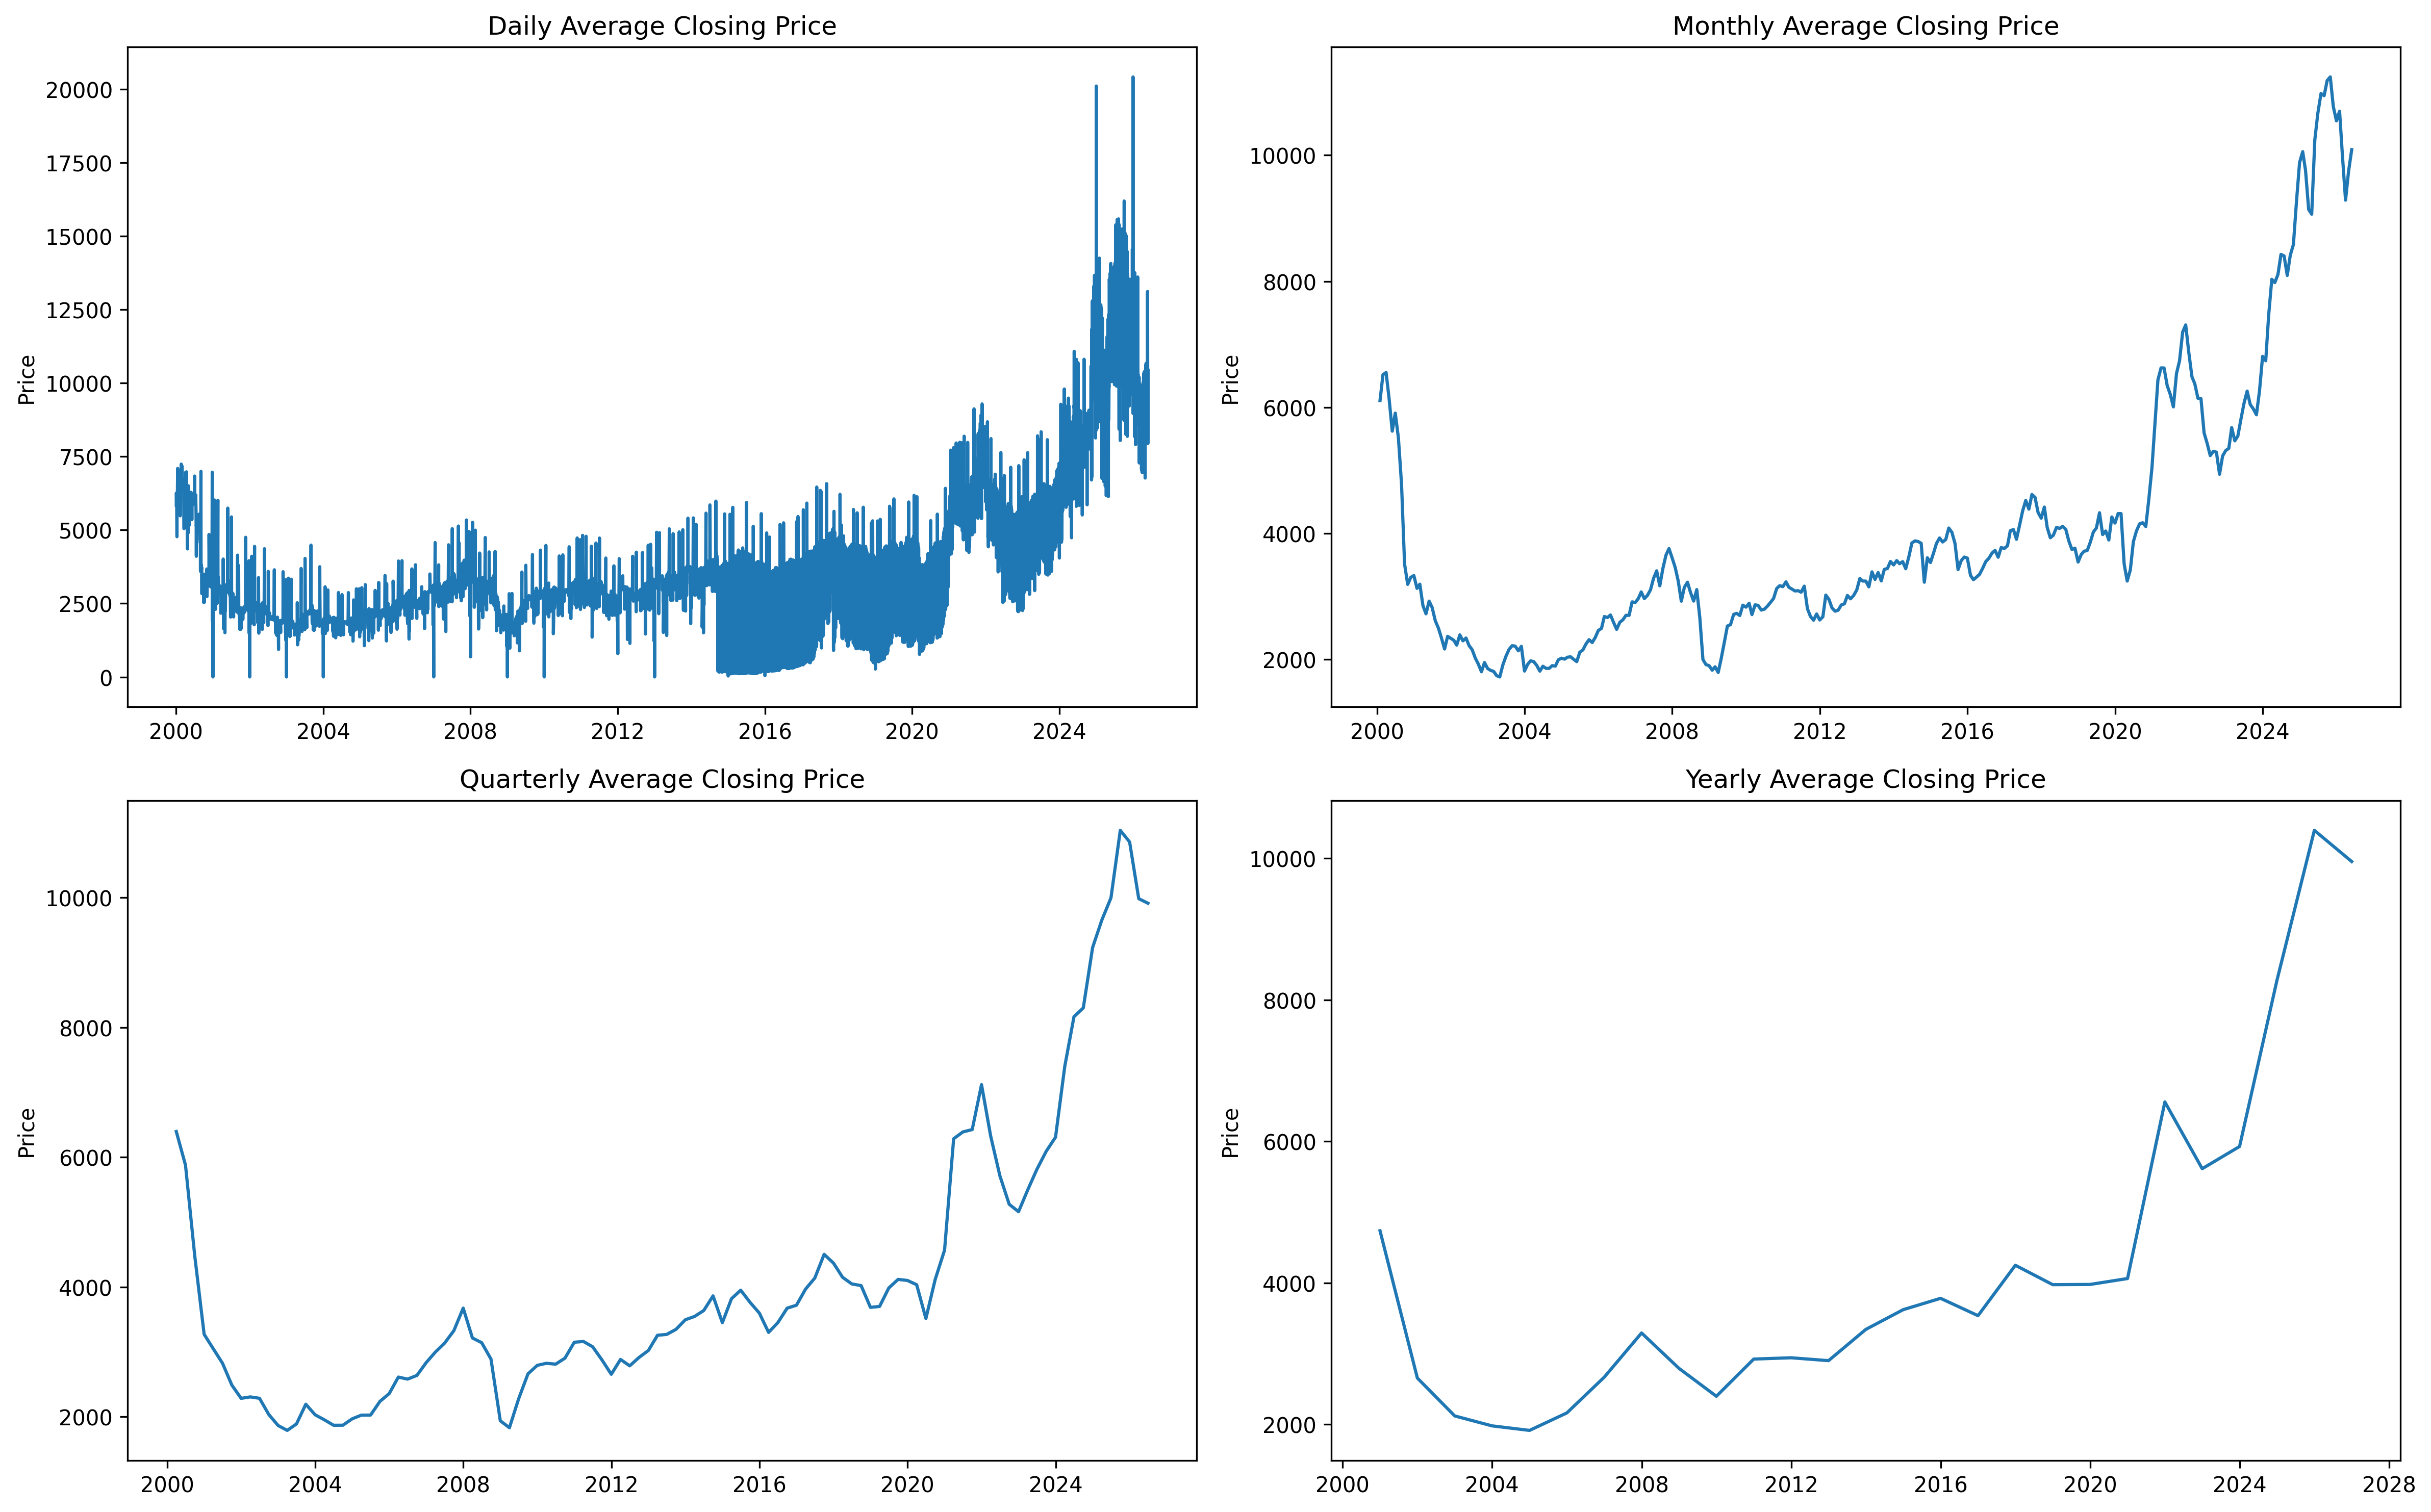
\includegraphics[width=\linewidth]{market_trends.png}  \caption{Average closing price aggregated at four frequencies: daily (top-left), monthly (top-right), quarterly (bottom-left), and yearly (bottom-right). Short-run noise diminishes progressively with coarser aggregation, revealing the underlying secular trend more clearly at each level.}
  \label{fig:ts_4panel}
\end{figure}

The daily series exhibits substantial short-term volatility, reflecting frequent market fluctuations and asset-specific movements. As the data is aggregated to monthly, quarterly, and yearly frequencies, these short-term variations become progressively smoother. Across all aggregation levels, an overall upward trend is evident, with periods of elevated volatility corresponding to major economic and financial events.

\subsection{Segmented Economic Period Analysis}

Figure~\ref{fig:ts_4periods} decomposes the full time series into four economically meaningful sub-periods.

\begin{figure}[H]
  \centering
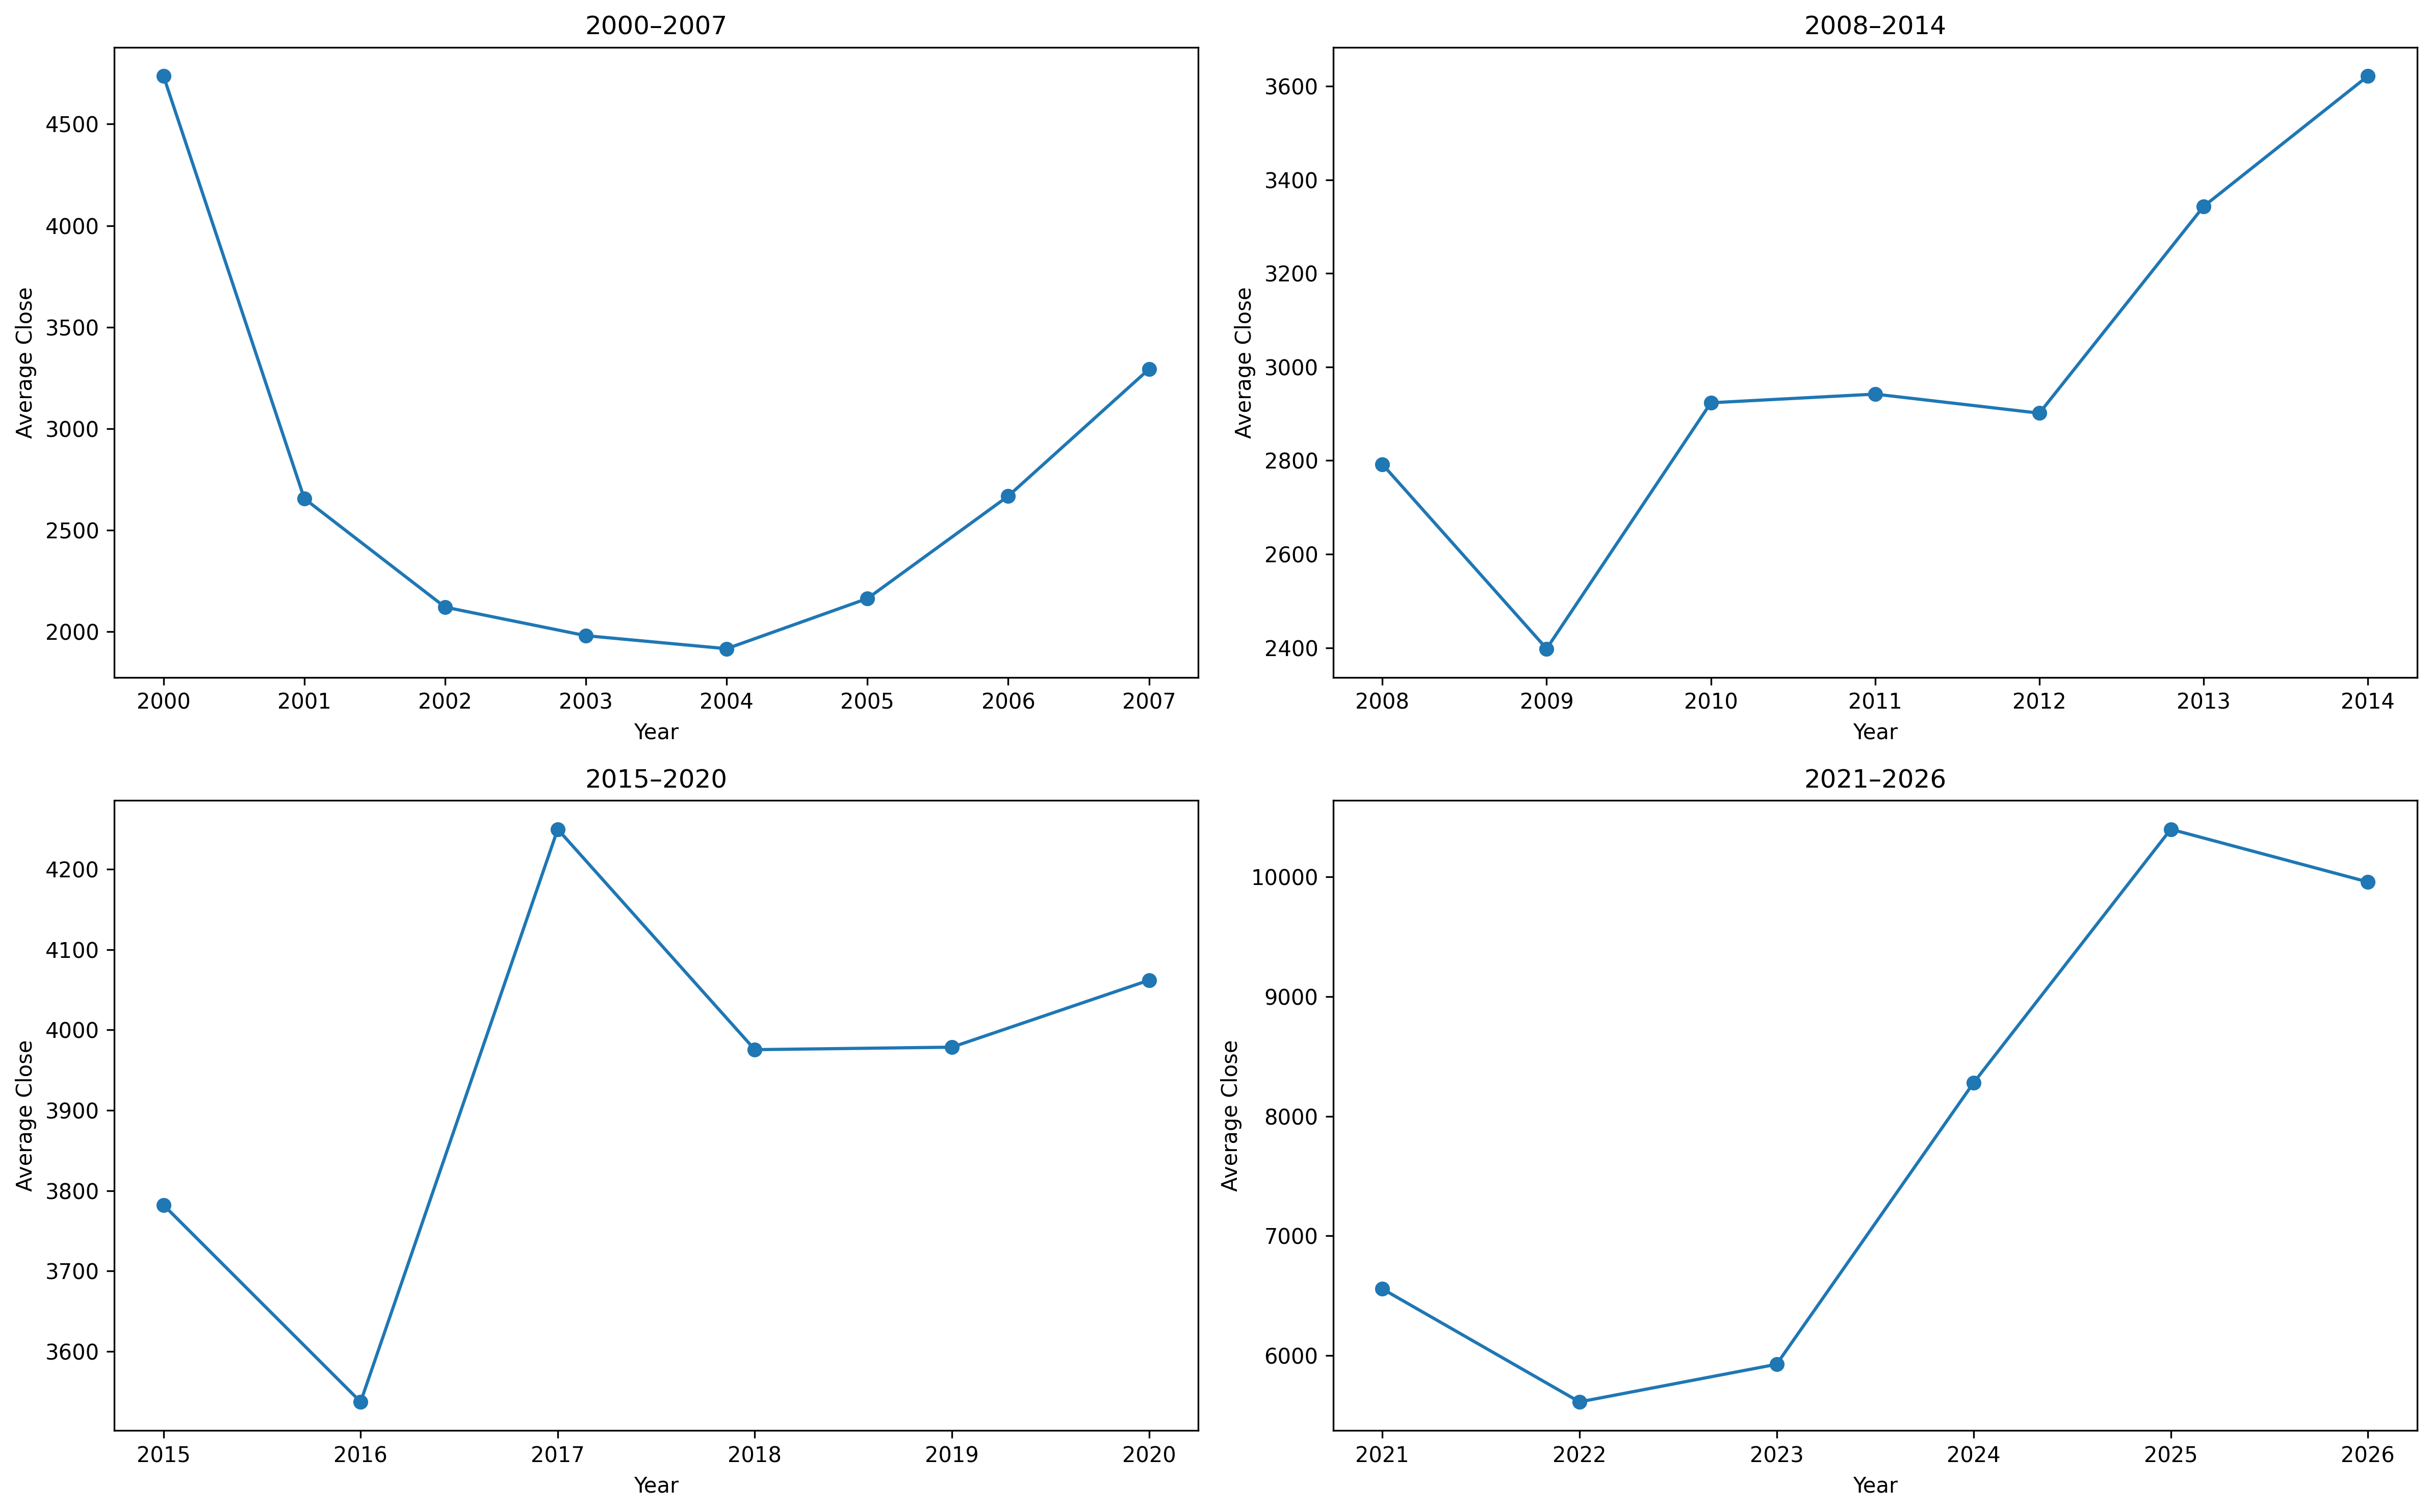
\includegraphics[width=\linewidth]{market_trends_2.png}  \caption{Yearly average closing price across four economic sub-periods. Each panel highlights a distinct market phase, from the Dot-Com correction (2000--2007) through the post-pandemic expansion (2021--2026).}
  \label{fig:ts_4periods}
\end{figure}

\textit{2000--2007 (Dot-Com Aftermath).} The market declined sharply from approximately 4,700 in 2000 to below 2,000 by 2004 as the technology bubble deflated. A gradual recovery followed, with prices recovering to approximately 3,300 by 2007.

\textit{2008--2014 (Global Financial Crisis and Recovery).} Average prices fell from approximately 2,800 in 2008 to 2,400 in 2009 during the GFC trough. The subsequent recovery was sustained and reached approximately 3,600 by 2014, driven by quantitative easing programs across major central banks.

\textit{2015--2020 (Pre-Pandemic Expansion).} This period was characterized by relative stability punctuated by a brief correction in 2016 and a sharp recovery in 2017--partly attributable to the first major cryptocurrency appreciation cycle. By 2020, moderate growth had resumed despite early-year pandemic uncertainty.

\textit{2021--2026 (Post-Pandemic Rally).} This sub-period exhibits the strongest growth trajectory of the entire dataset. Average closing prices rose from approximately 5,900 in 2023 to over 10,000 by 2025, driven by the pandemic-era monetary stimulus, sustained equity market expansion, and accelerating cryptocurrency market capitalization.

\subsection{Moving Average Trend Analysis}

Figure~\ref{fig:ma_chart} presents the monthly closing price series overlaid with 12-month and 24-month rolling averages.

\begin{figure}[H]
  \centering
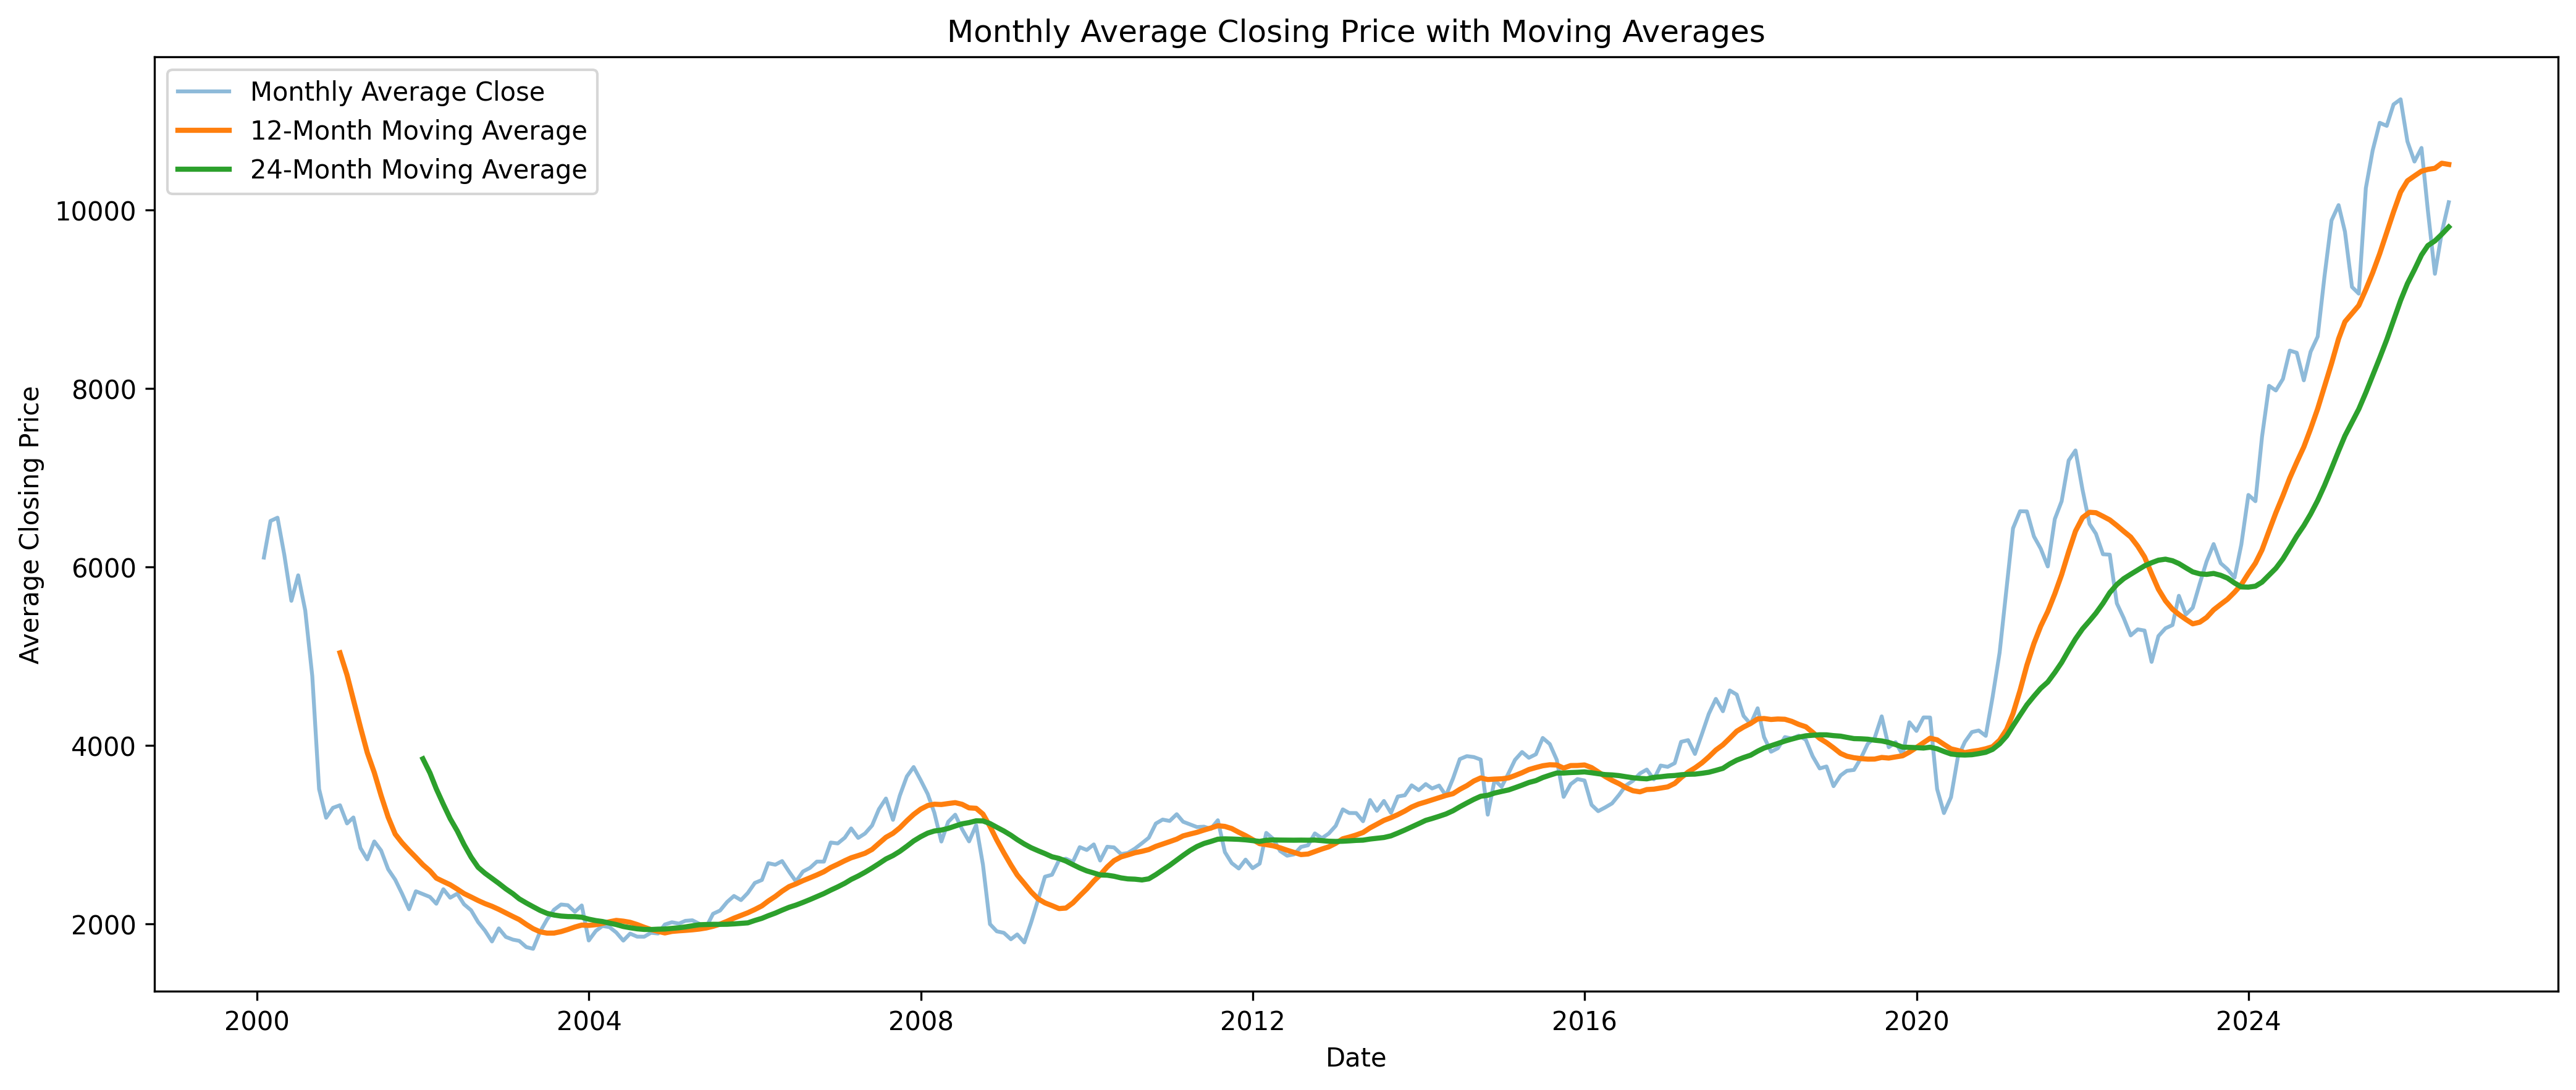
\includegraphics[width=\linewidth]{rolling_trends.png}  \caption{Monthly average closing price with 12-month and 24-month rolling moving averages (2000--2026). The 24-month MA provides a smooth representation of the secular upward trend, while temporary inversions of the 12-month MA against the 24-month MA coincide with the three major crisis episodes.}
  \label{fig:ma_chart}
\end{figure}

The 12-month moving average captures medium-term market movements and responds more quickly to changes in market conditions. The 24-month moving average offers a smoother representation of the underlying long-term trend by filtering out a greater portion of short-term volatility.

The chart reveals a significant decline in average closing prices during the early 2000s, followed by a period of gradual recovery and relatively stable growth through the following decade. Temporary downturns are visible around the 2008 GFC and the 2020 COVID-19 shock; both moving averages subsequently recover, confirming market resilience. From 2021 onward, both MAs exhibit a notably steeper upward slope, the steepest gradient in the full 26-year sample.

The divergence between the 12-month and 24-month moving averages serves as a useful proxy for medium-term momentum: periods where the 12-month MA lies above the 24-month MA correspond broadly to bullish phases, while inversions coincide with the three major crisis episodes.

\subsection{Correlation Analysis}

The Pearson correlation matrix computed for the five numerical features (Open, High, Low, Close, Volume) reveals two structurally distinct groups (Figure~\ref{fig:corr_heatmap}).

\begin{figure}[H]
  \centering
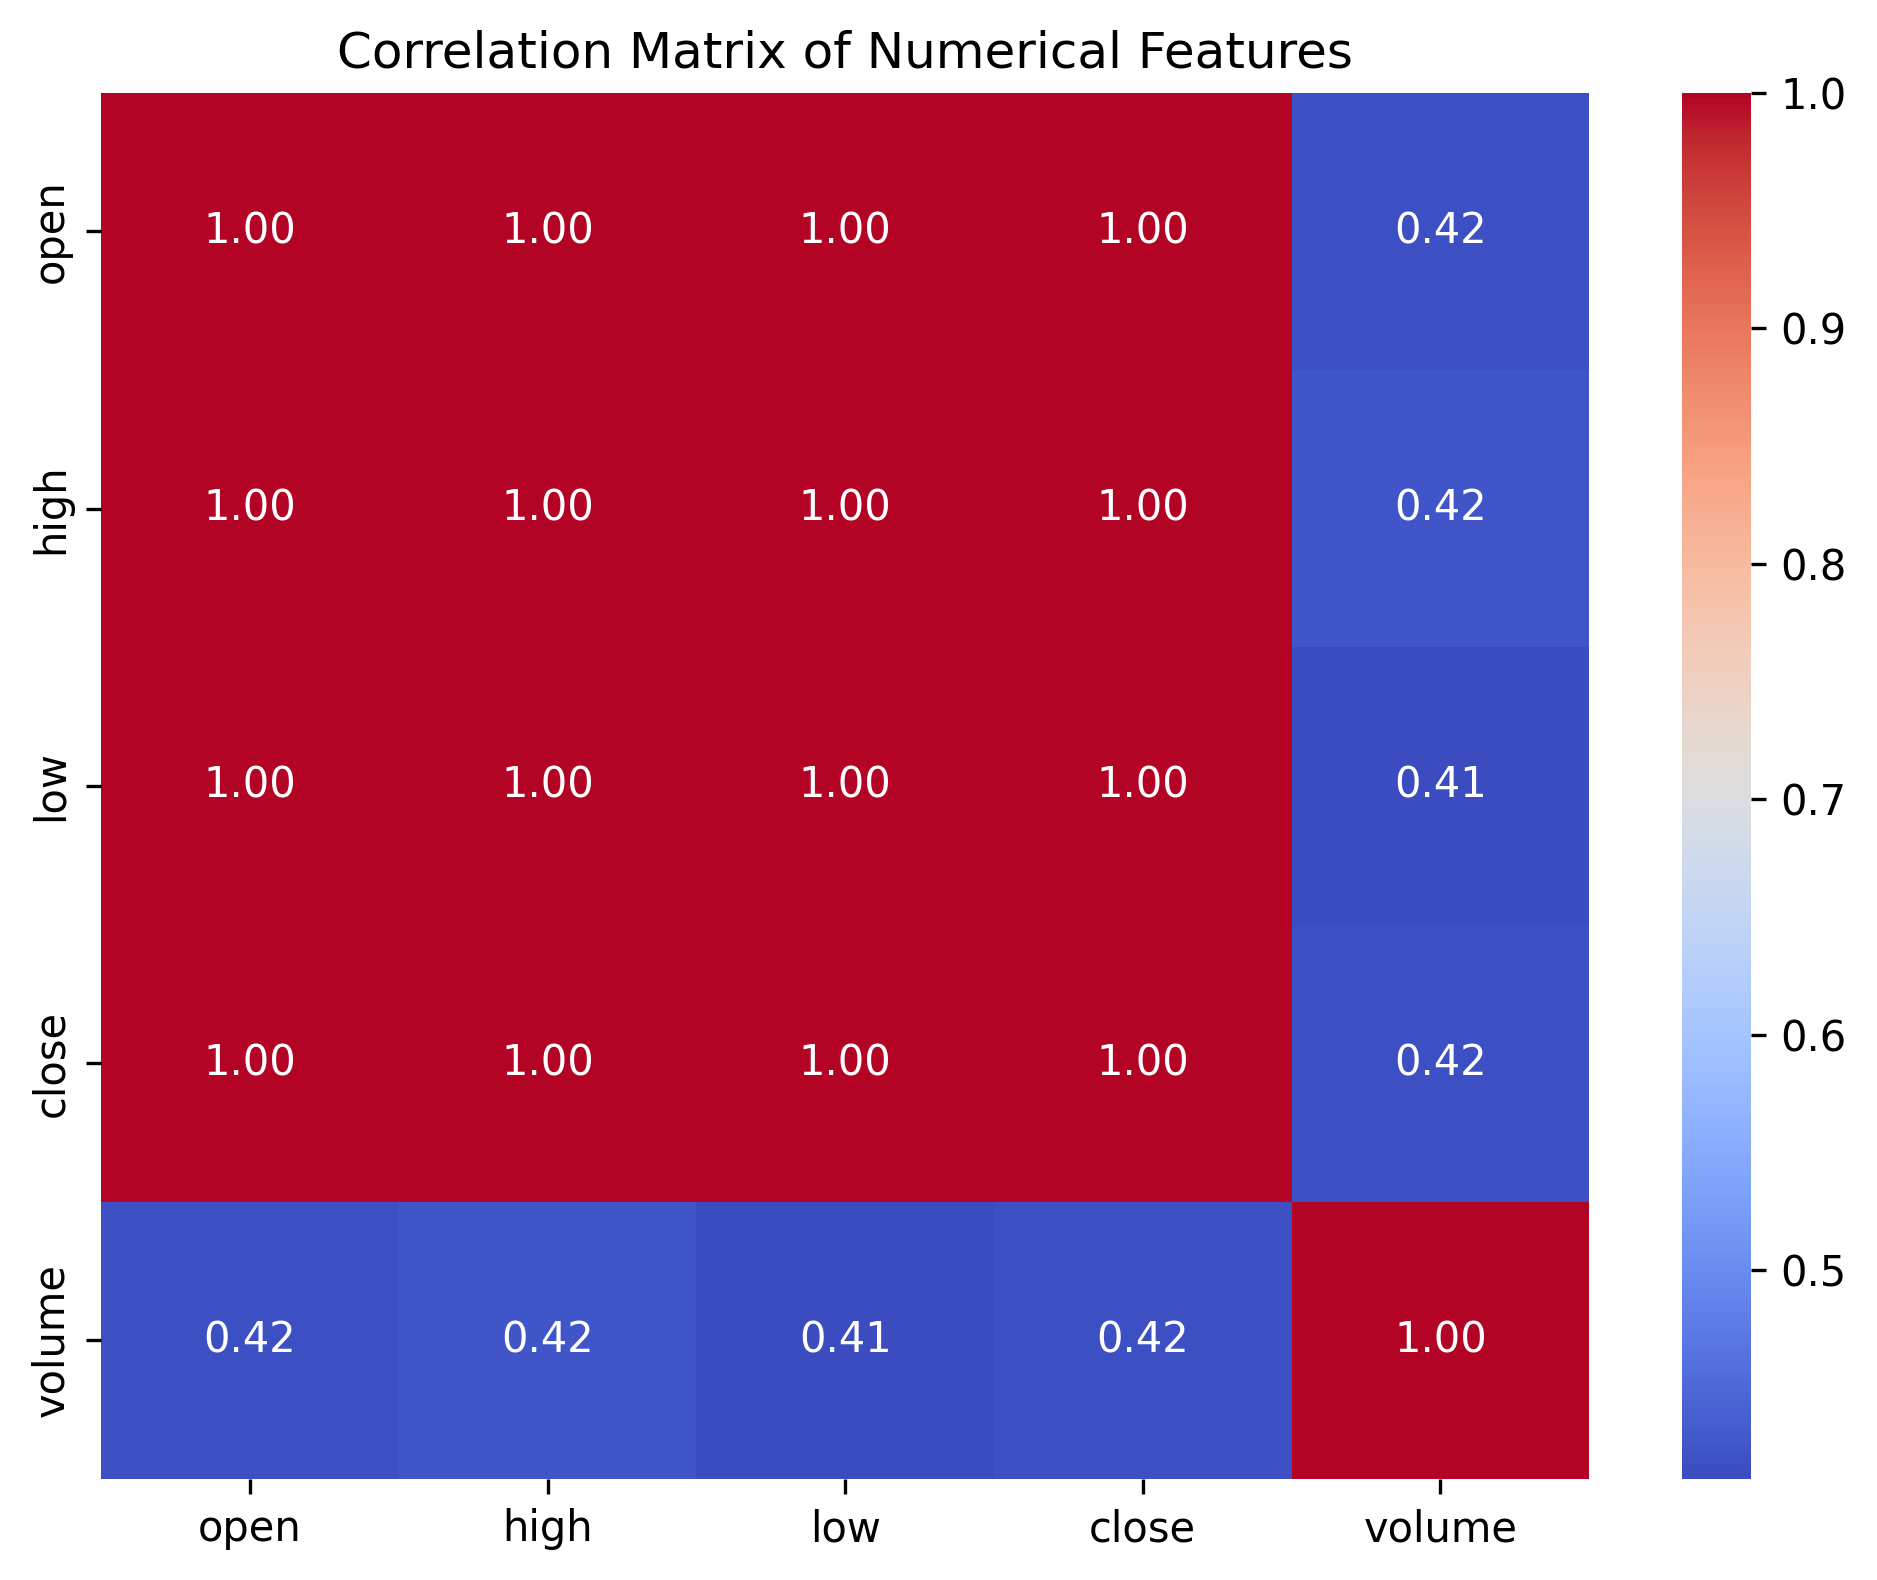
\includegraphics[width=\linewidth]{correlation_heatmap.png}  \caption{Pearson correlation heatmap for the five numerical features. OHLC variables form a near-perfect correlation cluster ($r > 0.999$), while trading volume is structurally decoupled from price ($|r| \approx 0.42$).}
  \label{fig:corr_heatmap}
\end{figure}

\begin{itemize}[leftmargin=1.2em, itemsep=1pt, topsep=2pt]
  \item \textbf{OHLC Cluster:} Open, High, Low, and Close are highly intercorrelated ($r > 0.999$ in all pairwise combinations), reflecting the mechanical constraint that within-day prices rarely diverge substantially from the opening level in a cross-asset aggregate over the long run.
  \item \textbf{Volume:} Trading volume exhibits substantially lower correlations with all price variables ($r \approx 0.41$--$0.42$), indicating that price level and trading intensity are structurally distinct phenomena. This finding is consistent with established empirical results in market microstructure literature.
\end{itemize}

The weak price-volume relationship is important when constructing predictive features: raw price levels are poor proxies for trading activity, and volume-based signals must be modeled independently.

\subsection{Major Market Events: Event-Period Analysis}

Segmenting the monthly time series at macroeconomic event boundaries confirms the qualitative pattern described above. Table~\ref{tab:event_summary} provides a structured summary of observed market behavior across major event periods.

\begin{table}[H]
\centering
\caption{Market Behavior During Major Economic Events}
\label{tab:event_summary}
\small
\begin{tabular}{@{}p{2.2cm}p{1.4cm}p{3.3cm}@{}}
\toprule
\textbf{Event} & \textbf{Period} & \textbf{Observed Effect} \\
\midrule
Dot-Com Crash    & 2000--2002 & Sharp equity decline; prolonged multi-year recovery \\
Post-GFC Shock   & 2007--2009 & Cross-asset drawdown; liquidity crisis \\
Pre-COVID Growth & 2009--2020 & Sustained bull market; QE-driven expansion \\
COVID Crash      & Q1 2020    & Rapid decline; fastest recovery on record \\
Post-COVID Rally & 2020--2026 & Strongest growth phase in full sample \\
\bottomrule
\end{tabular}
\end{table}

Each successive disruption was followed by a recovery that surpassed the prior peak, consistent with the long-run resilience hypothesis for diversified market portfolios.

%====================================================
% SECTION VI: KEY FINDINGS
%====================================================
\section{Key Findings}

The following findings are drawn from the analysis:

\begin{enumerate}[leftmargin=1.4em, itemsep=2pt, topsep=2pt]
  \item The dataset contains 187,611 records across 34 unique instruments spanning 26.4 years, with zero missing values and zero duplicate records.
  \item Seven high/low consistency anomalies were identified; all correspond to commodity instruments in 2009--2010 and were retained with documentation.
  \item The negative WTI Crude Oil price record of 21 April 2020 represents a valid historical event and was retained as-is.
  \item Stock indices represent the largest asset category by record count (63,610); cryptocurrencies the smallest (26,407).
  \item Cryptocurrencies exhibit the highest average daily trading volumes ($6.55 \times 10^{9}$), nearly seven times those of stock indices.
  \item Bitcoin and Ethereum collectively account for the two largest cumulative volumes in the dataset; six of the top ten volume-ranked assets are cryptocurrencies.
  \item Trading volume is highly right-skewed, with the lower quartile at zero and the upper quartile at $2.23 \times 10^{8}$.
  \item Global financial markets demonstrate a robust long-term upward trajectory spanning 2000--2026, confirmed at daily, monthly, quarterly, and yearly aggregations.
  \item The 2021--2026 sub-period exhibits the steepest growth gradient in the full sample, with average closing prices exceeding 10,000 by 2025.
  \item Major macroeconomic events generate temporary but quantifiable disruptions to the long-term trend; each recovery consistently establishes new price levels above prior peaks.
  \item The 24-month moving average confirms a smooth secular growth path largely unaffected by short-run volatility.
  \item OHLC price variables are near-perfectly intercorrelated ($r > 0.999$); trading volume is structurally decoupled ($r \approx 0.42$).
\end{enumerate}

%====================================================
% SECTION VII: CONCLUSION
%====================================================
\section{Conclusion}

This study presents a comprehensive exploratory analysis of global financial market data spanning 26 years and four major asset classes. Through a rigorous data quality pipeline, systematic temporal analysis across multiple aggregation horizons, moving average trend decomposition, correlation analysis, and event-based segmentation, a coherent and internally consistent picture of market dynamics emerges.

The central finding is that global markets exhibit strong long-term resilience: while major macroeconomic shocks - the Dot-Com Crash, the GFC, and COVID-19 - generate substantial temporary drawdowns, each recovery phase has produced new price highs, confirming the long-run upward trajectory of global capital markets. Concurrently, the rapid growth of cryptocurrency markets has introduced a new structural component characterized by extreme volume concentration and high return volatility, which must be accounted for in any multi-asset analytical framework.

The data cleaning phase, though revealing only minor quality issues, demonstrated best practices for financial data validation: systematic null checks, duplicate detection, type coercion, logical constraint testing, and explicit handling of economically significant anomalous observations rather than their mechanical removal.

These findings provide a robust empirical foundation for subsequent work including predictive modeling, volatility analysis, and portfolio optimization across multi-asset universes.

%====================================================
% SECTION VIII: FUTURE WORK
%====================================================
\section{Future Work}

Potential extensions of this research include:
\begin{itemize}[leftmargin=1.2em, itemsep=1pt, topsep=2pt]
  \item Machine learning-based forecasting of closing prices and trading volume using LSTM and Transformer architectures.
  \item GARCH and stochastic volatility modeling for risk quantification and tail-risk estimation.
  \item Cluster analysis of asset similarity based on rolling return profiles and drawdown patterns.
  \item Mean-variance and Black-Litterman portfolio optimization incorporating the multi-asset universe.
  \item Regime-switching models to formally identify and characterize bull/bear market phases.
  \item Sentiment-driven analysis integrating news and social media signals for cryptocurrency assets.
  \item Interactive market dashboards integrating the full analytical pipeline.
\end{itemize}

%====================================================
% REFERENCES
%====================================================
{\small
\begin{thebibliography}{5}

\bibitem{dataset}
Kaggle,
``Global Financial Markets Dataset,''
Available: \url{https://www.kaggle.com/},
Accessed: June 2026.

\bibitem{pandas}
Pandas Documentation,
``Pandas User Guide,''
Available: \url{https://pandas.pydata.org/docs/},
Accessed: June 2026.

\bibitem{numpy}
NumPy Documentation,
``NumPy User Guide,''
Available: \url{https://numpy.org/doc/stable/},
Accessed: June 2026.

\bibitem{matplotlib}
Matplotlib Documentation,
``Matplotlib Documentation,''
Available: \url{https://matplotlib.org/stable/},
Accessed: June 2026.

\bibitem{seaborn}
Seaborn Documentation,
``Seaborn Statistical Data Visualization,''
Available: \url{https://seaborn.pydata.org/},
Accessed: June 2026.

\end{thebibliography}
}

\end{document}